\documentclass[arbeit=studie,oneside,BCOR=12mm]{ArbeitRST}
% Die Option BCOR legt den Rand für die Bindekorrektur links fest
% (verschiebt das ganze Dokument nach rechts auf dem Papier, damit
% Platz zum Binden ist

% bib-Datei mit den Literaturangaben
% ==================================
\addbibresource{Literaturverzeichnis.bib}

\usepackage{float}
\usepackage{physics}
\usepackage{amsmath}
\usepackage{csvsimple}
\usepackage{mathtools}
\usepackage{todonotes}


% Zwei Parameter zum Verändern des Layouts
% ========================================
% \parindent -> Legt fest, mit welcher Einrückung jeder neue
%               Absatz beginnen soll
% \parskip -> Legt fest, wieviel vertikaler Abstand zwischen zwei
%             Absätzen liegen soll
%
% Tipp: Entweder parindent auf Null und parskip auf einen Wert
% ungleich Null (z.B. 2ex) oder umgekehrt. Beide Werte ungleich
% Null macht satztechnisch keinen Sinn. 1ex = Breite des 
% Buchstabens x
\setlength{\parindent}{0ex}
\setlength{\parskip}{2ex}



% Einige Einstellungen für das hyperref-Paket
% =========================================== 
% Hiermit können Links, Gleichungsnummern etc. farbig dargestellt
% werden was die Navigation im elektronischen Dokument vereinfacht. An
% dieser Stelle können Sie die Farbgebung anpassen. Druckversion bitte
% ohne farbige Links erstellen, siehe Option unten!
\hypersetup{
    unicode=false,          % non-Latin characters in Acrobat’s bookmarks
    pdftoolbar=true,        % show Acrobat’s toolbar?
    pdfmenubar=true,        % show Acrobat’s menu?
    pdffitwindow=false,     % window fit to page when opened
    pdfstartview={FitH},    % fits the width of the page to the window
    pdftitle={RST Vorlage}, % title
    pdfauthor={Author},     % author
    pdfsubject={Subject},   % subject of the document
    pdfcreator={Creator},   % creator of the document
    pdfproducer={Producer}, % producer of the document
    pdfkeywords={keyword1} {key2} {key3}, % list of keywords
    pdfnewwindow=true,      % links in new window
    colorlinks=true,        % false: boxed links; true: colored links
    linkcolor=blue,         % color of internal links (change box color with linkbordercolor)
    citecolor=green,        % color of links to bibliography
    filecolor=magenta,      % color of file links
    urlcolor=cyan           % color of external links
}

% Entfernt die farbigen Markierungen - bitte Druckversion mit dieser Option kompilieren
%\hypersetup{hidelinks}

   

% =================================================================
\begin{document}

% Titelseite
% ==========

% Name des Verfassers
\author{Julius Fiedler}

% Geburtsort
\geburtsort{Dresden}

% Geburtsdatum
\geburtsdatum{13. Oktober 1996}

% Titel der Arbeit
\title{Approximationsmethoden für dynamische Systeme auf Basis des Maschinellen Lernens}

% Untertitel
%\subtitle{}

% Angabe der Betreuer
\betreuer{Dr.-Ing. C. Knoll}


% Datum der Einreichung
\date{27. Oktober 2020}


% Zunächst für das Vorgeplänkel römische Seitenzahlen und einfacher Seitenstil
% ============================================================================
\pagenumbering{Roman}
\pagestyle{plain}


% Titelseite erstellen
\maketitle


% Selbstständigkeitserklärung
% ===========================

% Ort der Selbstständigkeitserklärung (Standard: Dresden)
\selbstort{Dresden}

% Datum der Selbstständigkeitserklärung (Standard: aktuelles Systemdatum)
\selbstdatum{27. Oktober 2020}

% Selbstständigkeitserklärung erstellen
\selbststaendigkeitserklaerung


% Kurzfassung / Abstract
% ======================
\kurzfassung{Systemmodelle sind eine Grundvoraussetzung in der Regelungstechnik. Um analytische Zusammenhänge verstehen zu können, sind White-Box-Modelle von Nöten. \textit{Sparse Identification of Nonlinear Dynamics} (SINDy) ist ein Verfahren, um die zugrundeliegenden Differentialgleichungen eines Systems zu bestimmen. SINDy wird an Systemen unterschiedlicher Komplexität getestet und es werden Richtlinien für eine effektive Nutzung abgeleitet. Es werden Methoden aufgezeigt, um die Genauigkeit des Algorithmus zu erhöhen und im Voraus bestehendes Wissen einfließen zu lassen. }{Having access to system models is essential in control theory. To understand the underlying analytical equations of a system, a white-box-model is needed. \textit{Sparse Identification of Nonlinear Dynamics} (SINDy) is a method to identify the governing equations of a system from its measurement data. SINDy is tested on systems of different complexity to establish guidelines for an effective use. Furthermore, techniques are shown to enhance the accuracy of the algorithm and make use of prior knowledge of the system.










}


% Inhaltsverzeichnis
% ==================
\tableofcontents

% Ggf. Symbolverzeichnis
% ======================
\chapter*{Verzeichnis der Formelzeichen \markboth{VERZEICHNIS DER FORMELZEICHEN}{}} \label{ch:Symbolverzeichnis}
\addcontentsline{toc}{chapter}{Verzeichnis der Formelzeichen}

\begin{table}[htbp]
\centering
\begin{tabular}{llp{9 cm}}
$C^r(n,k)$ & Kombination mit Wiederholung
$\varepsilon$ & Fehler der Moore-Penrose-Lösung\\
$\varepsilon_\text{r}$& relativer Fehler der identifizieren Koeffizienten\\
$\boldsymbol{f}$ & Systemdynamik\\
$F$ & Kraft, die auf den Wagen wirkt\\
$g$ & Erdbeschleunigung\\
$m$ & Anzahl der Messungen\\
$m_1$ & Masse des Wagens\\
$m_2$ & Masse am Ende des Pendels\\
$n$ & Anzahl der Zustände\\
$L$ & Anzahl der Ansatzfunktionen in $\Theta$\\
$\boldsymbol{p}$ & Parametervektor\\
$P$ & nominale Koeffizientenmatrix\\
$\varphi$ & Auslenkung des Pendels aus der unteren Ruhelage\\
$Q$ & identifizierte Koeffizientenmatrix\\ 
$R$ & Hilfsmatrix zur Berechnung von $\varepsilon_\text{r}$\\
$s$ & Länge des Pendels\\
$t$ & Zeit \\
$\theta$ & Gruppe von Ansatzfunktionen\\
$\Theta$ & $\Theta(X)$\\
$\Theta(X)$ & Bibliotheksmatrix aus Ansatzfunktionen, ausgewertet für alle von $X$\\
$\Theta^+$ & Moore-Penrose-Inverse von $\Theta$\\
$\Theta_\text{v}$ & verkleinerte Bibliotheksmatrix\\
$U$ & Unbekannte Funktion\\
$x$ & Position des Wagens\\
$\boldsymbol{x}(t)\in\mathbb{R}^n$ & Zustandsvektor\\
$X$ & Matrix der zeitlichen Verläufe der Zustandskomponenten\\
$\dot{X}$ & Matrix der zeitlichen Verläufe der Ableitungen der Zustandskomponenten\\
$\xi$ & Spalte von $\Xi$\\
$\Xi$ & Koeffizientenmatrix\\
$\Xi^\text{d}$ & dünn besetzte Koeffizientenmatrix\\
$\hat{\Xi}$ & verkleinerte Koeffizientenmatrix unter Nutzung von $\Theta_\text{v}$\\
$\Xi^n$ & Koeffizientenmatrix in den Dimensionen von $\Xi$ mit den Einträgen von $\hat{\Xi}$\\

\end{tabular}
\end{table}

\chapter*{Verzeichnis der Abkürzungen \markboth{VERZEICHNIS DER ABKÜRZUNGEN}{}} \label{ch:Abkürzungsverzeichnis}
\addcontentsline{toc}{chapter}{Verzeichnis der Abkürzungen}
\begin{table}[htbp]
\centering
\begin{tabular}{llp{9cm}}
DGL & Differentialgleichung \\
& \\
MKQ & Methode der kleinsten Quadrate\\
 & \\
SINDy & System Identification of Nonlinear Dynamics\\
STLSQ & Sequentially Thresholded Least Square
\end{tabular}
\end{table}


% Ggf. Abbildungsverzeichnis
% ==========================
\listoffigures


% Ggf. Tabellenverzeichnis
% ========================
%\listoftables\todo{raus}


% ========================
% Beginn Inhalt der Arbeit
% ========================

% Inhalt kann entweder in separate LaTeX-Dateien ausgelagert werden
% (hier: inhalt.tex) und dann mittels \input{} geladen werden...
% Darauf achten, dass pagenumbering und pagestyle richtig gesetzt werden
% (siehe Einträge in inhalt.tex)


%\chapter{Erläuterungen zur Klasse ArbeitRST}

% Ab hier arabische Seitenzählung und heading Seitenstil
\pagestyle{scrheadings}
\pagenumbering{arabic}

In den folgenden Abschnitten werden einige Erläuterungen zur \LaTeX-Dokumentenklasse \texttt{ArbeitRST.cls} gegeben werden. Diese basiert auf der Klasse \texttt{scrbook} aus dem KOMA-Script-Paket und kann daher mit Hilfe der Methoden aus diesem Paket modifiziert werden. Für nähere Informationen dazu sei auf die KOMA-Script-Anleitung\footnote{Diese kann unter der URL \url{http://www.ctan.org/pkg/koma-script} heruntergeladen werden.} und die Website
\begin{center}
	\url{http://www.komascript.de/}
\end{center}
verwiesen. 

Die wesentlichsten Änderungen gegenüber der ursprünglichen Klasse bestehen in einer angepassten Titelseite und der hinzugefügten Selbstständigkeitserklärung.



% ====================================================
\section{Informationen zu schriftlichen Arbeiten am RST}
Informieren Sie sich in der für Sie relevanten Prüfungsordnung über die \emph{Anzahl der geforderten Exemplare} die eingereicht werden müssen. Bitte beachten Sie, dass jedes dieser Exemplar die \emph{Aufgabenstellung} enthalten muss. Lassen Sie diese bitte beim Binden zwischen der Titelseite und der Selbstständigkeitserklärung einfügen. Eines der Exemplare muss dabei das \emph{originale}, vom Vorsitzenden des Prüfungsausschusses und dem verantwortlichen Hochschullehrer unterzeichnete, Dokument enthalten, bei den restlichen genügen Kopien. Bitte beachten Sie, dass die Arbeit \emph{einseitig} ausgedruckt werden muss. Ausschlaggebend für die fristgemäße Einreichung ist die \emph{Bestätigung des Prüfungsamtes}. Informieren Sie sich daher im \emph{Vorfeld} über die Öffnungszeiten am Abgabetag. Sollte das Prüfungsamt geschlossen haben, ist es in der Regel möglich mit den Mitarbeitern eine individuelle Vereinbarung zu treffen.


% ====================================================
\section{Die Titelseite}
Die Titelseite kann über die in Tabelle \ref{tab:titel} angegebenen Befehle angepasst werden.
\begin{table}[htbp]
\caption{Befehle zum Anpassen der Titelseite}
\label{tab:titel}
\begin{tabular}{lp{12cm}}
Befehl & Bedeutung\\
\toprule
\verb|\author| & legt den Namen des Autors der Arbeit fest\\
\verb|\geburtsdatum| & legt das Geburtsdatum des Autors fest\\
\verb|\geburtsort| & legt das Geburtsort des Autors fest\\
\verb|\title| & legt den Titel der Arbeit fest\\
\verb|\subtitle| & legt den Untertitel der Arbeit fest\\
\verb|\betreuer| & fügt einen Betreuer hinzu\\
\verb|\date| & legt das Einreichungsdatum der Arbeit fest -- \newline wird dieser Befehl nicht aufgerufen wird standardmäßig das zum Kompilationszeitpunkt eingestellte Systemdatum verwendet.\\
\bottomrule
\end{tabular}
\end{table}



% ====================================================
\section{Die Selbstständigkeitserklärung}
In der Selbstständigkeitserklärung werden automatisch der Typ der Arbeit, ihr Titel sowie der Name des Autors übernommen. Der Ort kann über den Befehl \verb|\selbstort| geändert werden, wobei standardmäßig "`Dresden"' verwendet wird. Das Datum ist standardmäßig identisch zum Einreichungsdatum, kann aber mit dem Befehl \verb|\selbstdatum| geändert werden.



% ====================================================
\section{Kurzfassung}
Eine Kurzfassung der Arbeit kann mit dem Befehl \verb|\kurzfassung{deutsch}{englisch}| eingefügt werden. Das erste Argument entspricht dabei der deutschen, das zweite der englischen Version.



% ====================================================
\section{Auswahl des Typs der Arbeit}
Zur Auswahl des Typs der Arbeit steht die Klassenoption \texttt{arbeit} zur Verfügung. Mit dieser können sie zwischen Diplom-, Master- und Studienarbeit sowie dem Bericht zum Forschungspraktikum auswählen:
\begin{table}[hbtp]%
\caption{Auswahl des Typs der Arbeit mittels Klassenoptionen}
\centering
\begin{tabular}{cc}
Diplomarbeit & \verb|\documentclass[arbeit=diplom]{ArbeitRST}|\\
Masterarbeit & \verb|\documentclass[arbeit=master]{ArbeitRST}|\\
Studienarbeit & \verb|\documentclass[arbeit=studie]{ArbeitRST}|\\
Bericht zum Forschungspraktikum & \verb|\documentclass[arbeit=forsch]{ArbeitRST}|
\end{tabular}
\label{}
\end{table}



% ====================================================
\section{Eingebundene Pakete}
In der Dokumentenklasse werden bereits einige \LaTeX-Pakete geladenen. Davon sind die zum Verfassen einer Arbeit möglicherweise relevanten in der Tabelle \ref{tab:pakete} aufgeführt. 
\begin{table}[htbp]%
\centering
\caption{Auswahl eingebundener Pakete}
\label{tab:pakete}
\begin{tabular}{p{3.6cm}p{11.4cm}}
amsmath, amssymb, \newline amsfonts, amsthm & Pakete zum Satz mathematischer Formeln, Dokumentation finden sie unter \newline\url{http://www.ams.org/publications/authors/tex/amslatex},\newline besonders empfehlenswert ist der "`Short Math Guide for \LaTeX"'\\
booktabs & ermöglicht das Setzen "`schöner"' Tabellen, Dokumentation unter \url{http://ctan.org/pkg/booktabs}\\
cite & verbessert einige Aspekte des Zitierens, Dokumentation unter \newline\url{http://ctan.org/pkg/cite}\\
caption, subcaption & Pakete zum Anpassen der Unter- und Überschriften von Tabellen, Grafiken etc., Dokumentation unter \newline\url{http://ctan.org/pkg/caption} \newline\url{http://ctan.org/pkg/subcaption}
\end{tabular}
\end{table}\\
Neben diesen Paketen wird das Paket \verb|hyperref| (\url{http://ctan.org/pkg/hyperref}) zur farbigen Hervorhebung von Verweisen, Links etc.\ eingebunden. Bitte deaktivieren Sie diese Markierungen vor dem Ausdrucken mit Hilfe des Befehls
\begin{center}
\verb|\hypersetup{hidelinks}|.
\end{center}



% ====================================================
\section{Zusätzliche Makros}
In die Dokumentenklasse \texttt{ArbeitRST} wurden einige Makros aufgenommen, die sich bei der Arbeit mit \LaTeX{} als nützlich erwiesen haben.
\begin{table}[htbp]
\centering
\caption{Zusätzliche Makros und Umgebungen}
\begin{tabular}{ccp{9cm}}
Syntax & Ausgabe & Beschreibung\\
\toprule
\texttt{\textbackslash vect\{a\}} & $\vect{a}$ & Umschaltung auf fette Schriftart im Mathemodus-- oft für Vektoren genutzt\\[2ex]
\texttt{\textbackslash diag(a,\textbackslash ldots,z)} & $\diag(a,\ldots,z)$ & Nützlich zur Definition von Diagonalmatrizen\\[2ex]
\texttt{\textbackslash diff[n]\{q\}\{t\}} & $\diff[n]{q}{t}$ & Ableitungen darstellen\\[2ex]
\texttt{\textbackslash partiell[n]\{q\}\{t\}} & $\partiell[n]{q}{t}$ & partielle Ableitungen darstellen\\[2ex]
\texttt{\textbackslash dr} &$\dr$ &Aufrechtes d für Integrale ($\int f(t) \dr t$)\\[2ex]
\texttt{\textbackslash Reals} & $\Reals$ & Körper der reellen Zahlen\\[2ex]
\texttt{\textbackslash Compl} & $\Compl$ & Körper der komplexen Zahlen\\[2ex]
\texttt{\textbackslash Real(a)} & $\Real(a)$ & Realteil von $a$\\[2ex]
\texttt{\textbackslash Imag(a)} & $\Imag(a)$ & Imaginärteil von $a$\\[2ex]
\texttt{\textbackslash norm\{a\}} & $\norm{a}$ & Norm von $a$\\[2ex]
\texttt{\textbackslash abs\{a\}} & $\abs{a}$ & Betrag von $a$\\[2ex]
\texttt{\textbackslash skalprod\{a\}\{b\}} & $\skalprod{a}{b}$ & Skalarprodukt von $a$ und $b$\\[2ex]
\texttt{\textbackslash grad(a)} & $\grad(a)$ & Gradient von $a$\\[2ex]
\texttt{\textbackslash div(a)} & $\div(a)$ & Divergenz von $a$\\
\bottomrule
\end{tabular}
\end{table}


Neben diesen Makros wurden Umgebungen zum Erzeugen von Definitionen (\verb|definition|), Beispielen (\verb|beispiel|), Lemmata (\verb|lemma|) und Bemerkungen (\verb|bemerkung|) definiert.

\begin{table}[htbp]%
\centering
\caption{Beispiele der vordefinierten Umgebungen}
\begin{tabular}{p{8cm}p{7cm}}
Syntax & Ausgabe\\
\toprule
\begin{verbatim}
\begin{definition}[Beispiel]
Beispiel für eine Definitionsumgebung
\end{definition}
\end{verbatim}
&
\begin{definition}[Beispiel]
Beispiel für eine Definitionsumgebung
\end{definition}
\\
\begin{verbatim}
\begin{beispiel}[Beispiel]
Beispiel für eine Beispielumgebung
\end{beispiel}
\end{verbatim}
&
\begin{beispiel}[Beispiel]
Beispiel für eine Beispielumgebung
\end{beispiel}
\\
\begin{verbatim}
\begin{lemma}[Beispiel]
Beispiel für eine Lemmaumgebung
\end{lemma}
\end{verbatim}
&
\begin{lemma}[Beispiel]
Beispiel für eine Lemmaumgebung
\end{lemma}
\\
\begin{verbatim}
\begin{bemerkung}[Beispiel]
Beispiel für eine Bemerkungsumgebung
\end{bemerkung}
\end{verbatim}
&
\begin{bemerkung}[Beispiel]
Beispiel für eine Bemerkungsumgebung
\end{bemerkung}\\
\bottomrule
\end{tabular}
\end{table}



% ====================================================
\section{Weitere Informationen}
Da \LaTeX\ seine Funktionalität im wesentlichen durch frei verfügbare Pakete erhält, ist es günstig eine Distribution zu installieren, die bereits die wesentlichen Pakete enthält und das Hinzufügen weiterer Pakete vereinfacht. Für Windows existiert beispielsweise MiKTeX (\url{http://miktex.org/}) und für Linux TeX Live (\url{http://www.tug.org/texlive/}). Zum Erstellen von \LaTeX-Dokumenten unter Windows hat sich das Programm TeXnicCenter (\url{http://www.texniccenter.org/}), vor allem in Verbindung mit dem Sumatra PDF-Betrachter (\url{http://blog.kowalczyk.info/software/sumatrapdf}), als sehr nützlich erwiesen. Unter Linux gilt dasselbe für das Programm Kile (\url{http://kile.sourceforge.net/}). Zum Erstellen und Verwalten von Bibtex-Dateien wurden gute Erfahrungen mit JabRef (\url{http://jabref.sourceforge.net/}) gemacht. Es existieren zahlreiche Bücher zum Umgang mit \LaTeX, von denen an dieser Stelle nur \cite{MittelbachGoosens05} aufgeführt wird.


%%% Local Variables:
%%% mode: latex
%%% TeX-master: "ArbeitRST"
%%% End:



% ...oder man schreibt direkt in dieser Datei (weniger übersichtlich)


% Ab hier Reinschrift
\chapter{Einleitung}
\pagenumbering{arabic}
\section{Motivation}
Für viele regelungstechnische Anwendungen ist die Kenntnis von Systemmodellen erforderlich. Unter Nutzung von Methoden des maschinellen Lernens können aus Messdaten Modelle erzeugt werden, die das Verhalten des Systems widerspiegeln können. Oft handelt es sich um Black-Box-Modelle, die zwar das Eingangs-Ausgangs-Verhalten des Systems wiedergeben, jedoch keinen Aufschluss zu den zugrunde liegenden Differentialgleichungen liefern können. Diese mathematischen Zusammenhänge können jedoch essenziell im Verständnis und im Umgang mit komplexen Systemen sein. In dieser Arbeit wird die Methode \textit{Sparse Identification of Nonlinear Dynamics} (SINDy) untersucht, die verspricht die Systemdifferentialgleichungen aus Messdaten des Systems zu rekonstruieren. 

\section{Präzisierung der Aufgabenstellung}
Aus den existierenden Methoden zur Systemidentifikation sollen vielversprechende Kandidaten ausgewählt werden. Diese sollen während der Literaturrecherche auf Eignung und Implementierbarkeit geprüft werden. 
Anschließend sollen wichtige Ergebnisse aus der Literatur reproduziert und weitere Beispielsysteme steigender Komplexität übertragen werden. 
Dabei soll der Einfluss der zur Verfügung stehenden Freiheitsgrade herausgearbeitet werden.


\chapter{Der SINDy-Algorithmus}
\label{cha:sindy}
\section{Vorbetrachtungen} 

Sparse Identification of Nonlinear Dynamics (SINDy) ist eine Methode, um aus den Messdaten eines Systems auf dessen Systemdifferentialgleichungen zu schließen. Die zugrundeliegende Annahme ist, dass die zu identifizierende Funktion in einem geeigneten Raum an Basisfunktionen \textit{dünn besetzt} ist. Betrachtet man beispielsweise die Funktion
\begin{equation}
\diff{x}{t} = f(x) = \begin{bmatrix} f_1(x)\\ f_2(x)\\ \end{bmatrix}
=\begin{bmatrix} 1+2x_1+x_1x_2^2 \\ x_1^3-3x_2\\ \end{bmatrix},
\end{equation}
so ist leicht zu erkennen, dass $f$ in Bezug auf die Basis von Polynomen aus zwei Variablen (z.B. $f_1(x)=\sum_{i=0}^{\infty}\sum_{j=0}^{\infty}a_{ij}x_1^ix_2^j$) dünn besetzt ist. Nur eine sehr geringe Zahl der Koeffizienten $a_{ij}$ ist ungleich null. 
Die dem Algorithmus zur Verfügung gestellten Basisfunktionen werden zu einer Bibliothek zusammengefasst. Hieraus werden mittels Regression diejenigen Ansatzfunktionen ausgewählt, deren Linearkombination die Funktion $f$ am besten repräsentiert. Es ist einsichtig, dass die Auswahl der Bibliotheksfunktionen eine entscheidende Rolle für den Erfolg der Methode spielt. Daher ist es günstig, wenn man bereits weiß, welche Funktionsklassen zu identifizieren sind, um die Bibliothek geeignet auszulegen. Wie der Methodenname suggeriert, können mit SINDy auch nichtlineare Funktionen identifiziert werden. 
\section{Funktionsweise der Methode}
Sei $f\left(x(t)\right) = \diff{x(t)}{t}$ das zu identifizierende Differentialgleichungssystem mit dem Zustandsvektor $x(t) = [x_1(t), x_2(t), ... , x_n(t)]^T \in\mathbb{R}^n$.
Für die Anwendung von SINDy benötigt man die Messdaten aller Zustandsgrößen zu den Zeitpunkten $t_1, t_2, ..., t_m$. Zusätzlich müssen die zeitlichen Ableitungen der Zustände an den gegebenen Zeitpunkten gegeben sein, entweder durch direkte Messung oder durch numerische Approximation. Die Daten werden wie folgt angeordnet: 
\begin{align}
X &= \begin{bmatrix}
		x_1(t_1) & x_2(t_1) & \dots & x_n(t_1) \\
		x_1(t_2) & x_2(t_2) & \dots & x_n(t_2) \\
		\vdots   & \vdots   & 		& \vdots \\ 
		x_1(t_m) & x_2(t_m) & \dots & x_n(t_m)
	\end{bmatrix} \in \mathbb{R}^{m\times n},
	\\
	\dot{X} &= \begin{bmatrix} 
		\dot{x}_1(t_1) & \dot{x}_2(t_1) & \dots & \dot{x}_n(t_1) \\
		\dot{x}_1(t_2) & \dot{x}_2(t_2) & \dots & \dot{x}_n(t_2) \\
		\vdots 		   & \vdots 		& 		& \vdots \\
		\dot{x}_1(t_m) & \dot{x}_2(t_m) & \dots & \dot{x}_n(t_m)
	\end{bmatrix}  \in \mathbb{R}^{m\times n}.
\end{align}
Nun muss man die Bibliothek $\Theta$ an Funktionen konstruieren, durch welche $f$ dargestellt werden soll. 
Die Spalten der Bibliotheksmatrix repräsentieren die gewählten Ansatzfunktionen, angewendet auf die Datenmatrix $X$ 
\begin{equation}
\Theta(X) = \begin{bmatrix}
		\mid & \mid & & \mid \\
		\theta_1(X) & \theta_2(X) & \dots & \theta_\ell(X) \\
		\mid & \mid & & \mid 
	\end{bmatrix}\in\mathbb{R}^{m\times L}.
\end{equation} 
Wählt man beispielsweise für $\theta_1$ die Sinusfunktion und für $\theta_2$ Monome zweiten Grades so ergeben sich 
\begin{align}
\theta_1(X) &= \begin{bmatrix}
		\mid 	  & \mid     		  &          & \mid             \\
		\sin(x_1(t)) & \sin(x_2(t))   & \dots    & \sin(x_n(t)) \\
		\mid      & \mid     		  &          & \mid              
	\end{bmatrix},\\
\theta_2(X) &= \begin{bmatrix}
		\mid & \mid & & \mid & \mid & & \mid \\
		x_1(t)^2 & x_1(t)x_2(t) & \dots & x_2(t)^2 & x_2(t)x_3(t) & \dots & x_n^2(t) \\
		\mid & \mid & & \mid & \mid & & \mid
	\end{bmatrix},	
\end{align}
wobei die Rechenoperationen alle elementweise zu lesen sind. \\
Gesucht sind nun Linearkombinationen von Bibliotheksfunktionen, sodass gilt
\begin{equation}
f_i(x) = \Theta(x^T)\xi_i.
\end{equation}
Fasst man alle $\xi_i$ in eine Koeffizientenmatrix $\Xi\in\mathbb{R}^{L\times n}$ zusammen, so ergibt sich das zu lösende Problem zu 
\begin{equation}
\dot{X} \approx \Theta(X)\Xi. \label{eq:Minimierungsproblem}
\end{equation}
\cite{Brunton2016}\\

\section{Lösen des Minimierungsproblems}
Das Lösen des Gleichungssystems \eqref{eq:Minimierungsproblem} ist die Kernaufgabe des Algorithmus. Das Gleichungssystem besitzt $m\cdot n$ Gleichungen ($m\text{ } \hat{=}$ Anzahl Messungen) und $L\cdot n$ Unbekannte ($L\text{ } \hat{=}$ Anzahl Ansatzfunktionen). Unter der Annahme, dass die Anzahl der Messungen ausreichend groß ist, handelt es sich um ein überbestimmtes Gleichungssystem. Es existieren verschiedene Optimierungsverfahren, um dieses Problem der Form
\begin{equation}
Ax=b
\end{equation}
zu lösen. In dieser Arbeit wurde hauptsächlich mit einer rekursiven Methode der kleinsten Quadrate (MKQ) gearbeitet. Sparse Relaxed Regularized Regression (SR3) wird zum Vergleich herangezogen. Der in dieser Arbeit entwickelte vereinfachte Algorithmus verwendet die erste Methode. \todo{Quelle?}
\section{Rekursive Methode der kleinsten Quadrate}
\label{sec:rMKQ}
Eine weit verbreitete Strategie zur Lösung überbestimmter Gleichungssysteme der Form
\begin{equation}
\dot{X} = \Theta\Xi
\end{equation} ist die Methode der kleinsten Quadrate. Dabei wird die Moore-Penrose-Inverse von $\Theta$ berechnet
\begin{equation}
\Theta^{+} = (\Theta^T\Theta)^{-1}\Theta^T.
\end{equation}
Die Moore-Penrose-Lösung
\begin{equation}
\Xi = \Theta^+\dot{X}
\end{equation}
minimiert dabei den Fehler
\begin{equation}
\epsilon = \norm{\Theta(X)\Xi-\dot{X}}_2. \label{eq:Fehler_MKQ}
\end{equation} 
Der Algorithmus beginnt mit dieser Näherungslösung für die Koeffizientenmatrix $\Xi$.
Um die Forderung nach einer dünnbesetzten Matrix umzusetzen, werden anschließend alle Koeffizienten, deren Betrag unter einem festgelegten Grenzwert liegt, zu Null gesetzt.
\begin{equation}
\Xi_\text{dünn, ij} = \begin{cases} 0 & |\Xi_\text{ij}| < \lambda\\
\Xi_\text{ij} & \text{sonst} 
\end{cases} ,\quad 1 \leq i \leq L, \quad 1\leq j \leq n \label{eq:make_sparse}
\end{equation}
Jeder nicht negative Koeffizient $\Xi_\text{dünn, ij}$ repräsentiert eine im Differentialgleichungssystem vorkommende Ansatzfunktion. Allerdings sind die Koeffizienten $\Xi_\text{dünn}$ fehlerhaft, da sie auf Basis der nicht vorkommenden Funktionen berechnet wurden. Es bietet sich an, die Koeffizientenmatrix $\Xi$ erneut zu berechnen, unter Nutzung des Wissens über welche Ansatzfunktionen in der Differentialgleichung (DGL) vorkommen.

Für jede Zeile der DGL wählt man diejenigen Spalten der Bibliotheksmatrix aus, die für Funktionen stehen, die nach \ref{eq:make_sparse} in dieser Zeile vorkommen. Dann kann man die Koeffizientenmatrix spaltenweise wie folgt berechnen (der Index a steht für Auswahl, die Indices der $\theta$ sind willkürlich gewählt):
\begin{subequations}
\begin{equation}
\dot{X}_i = 	\left(\begin{array}{c} 
      					 \mid \\
      					 \dot{x}_i(t)\\ 
      					 \mid 
    				\end{array}\right) \in \mathbb{R}^{m}
\end{equation}
\begin{equation}
\Theta_\text{a}(X) = \begin{bmatrix}
		\mid & \mid &  \mid &\\
		\theta_2(X) & \theta_5(X) & \theta_7(X) &\dots\\
		\mid & \mid &  \mid &
	\end{bmatrix}\in\mathbb{R}^{m\times l}.
\end{equation}
\begin{equation}
\hat{\Xi}_i = \xi_i \in\mathbb{R}^{l} = \Theta_\text{a}^+\dot{X}_i \label{eq:xi_select}
\end{equation}
\end{subequations}
Die Spalten $\hat{\Xi}_i$ können zu einer Matrix $\hat{\Xi}$ zusammengesetzt werden. Anschließend muss diese auf  $\Xi_\text{neu}\in\mathbb{R}^{L\times n}$ vergrößert und an den entsprechenden Stellen mit Nullen aufgefüllt werden: 
\begin{equation}
\Xi_\text{neu, ij} = \begin{cases}
						0 & |\Xi_\text{ij}| < \lambda\\
						\hat{\Xi}_\text{kj}, 1\leq k \leq l  & \text{sonst}

\end{cases}. \label{eq:reshape} % ist das mathematisch sauber?
\end{equation}
Allerdings besteht die Möglichkeit, dass $\Xi_\text{neu}$ durch die erneute Berechnung Einträge unterhalb des Grenzwertes besitzt.
Daher werden die Schritte \ref{eq:make_sparse}, \ref{eq:xi_select} und \ref{eq:reshape} solange wiederholt, bis in \ref{eq:make_sparse} $\Xi_\text{dünn} = \Xi$ gilt, also bis die Koeffizientenmatrix nicht mehr verändert wird. Es werden somit iterativ immer mehr Ansatzfunktionen ausgeschlossen. Damit gilt am Ende
\begin{subequations}
\begin{equation}
\dot{X} \approx \Theta(X)\Xi
\end{equation}
und somit
\begin{equation}
\dot{x} = f(x) \approx \Xi^T\left(\Theta(x^T)\right)^T,
\end{equation}
wobei $\Xi$ dünn besetzt ist.

\end{subequations}















\chapter{Durchführung von Tests}
\section{Vorstellung der Implementationen}
Neben dem in Abschnitt \ref{sec:rMKQ} vorgestellten vereinfachten Algorithmus werden zwei weitere Implementationen der SINDy-Methode untersucht. De Silva et al. \cite{desilva2020} haben SINDy in \textit{Python} (PySINDy) implementiert, während Rackauckas et al.\cite{Rackauckas2020} die SINDy-Implementation der DataDrivenDiffEq-Bibliothek in \textit{Julia} nutzen. Die drei Algorithmen sind sich im Aufbau sehr ähnlich und folgen dem in Kapitel \ref{cha:sindy} beschriebenen Ablauf. Jedoch unterscheiden sich die Algorithmen in der Lösungsstrategie des überbestimmten Gleichungssystems \eqref{eq:Axeqb}. PySINDy verwendet das Cholesky-Verfahren \cite{Krishnamoorthy2011}, während die Julia-Implementation die QR-Faktorisierung \cite{Martinsson2015} anwendet. 
\section{Vorstellung der Testsysteme}
Für den Vergleich der Implementationen werden drei verschiedene Differentialgleichungssystem betrachtet, deren Parameter es zu identifizieren gilt.

Das Lotka-Volterra-System
\begin{equation}
\begin{aligned}
\dot{x} &= \alpha x +\beta xy\\
\dot{y} &= \gamma y + \delta xy 
\end{aligned}
\end{equation}
mit den Nominalparametern
\begin{equation}
p_\text{LV}=\left(\begin{array}{c}
		\alpha\\\beta\\\gamma\\\delta
\end{array}\right) 
= \left(\begin{array}{c}
		1.3\\ -0.9\\ 0.8\\ -1.8
\end{array}\right).
\end{equation}

Das Lorenz-System
\begin{equation}
\begin{aligned}
\dot{x} &= \alpha(y-x)\\
\dot{y} &= x(\beta - z) -y\\
\dot{z} &= xy-\gamma z
\end{aligned}
\end{equation}
mit den Nominalparametern
\begin{equation}
p_\text{L}=\left(\begin{array}{c}
		\alpha\\\beta\\\gamma
\end{array}\right) 
= \left(\begin{array}{c}
		10\\ 28\\ \frac{8}{3}
\end{array}\right).
\end{equation}

Das Rössler-System
\begin{equation}
\begin{aligned}
\dot{x} &= -y-z\\
\dot{y} &= x+\alpha y\\
\dot{z} &= \beta + (x-c)z
\end{aligned}
\end{equation}
mit den Nominalparametern
\begin{equation}
p_\text{R}=\left(\begin{array}{c}
		\alpha\\\beta\\\gamma
\end{array}\right) 
= \left(\begin{array}{c}
		0.2\\ 0.1\\ 5.3
\end{array}\right).
\end{equation}

Ausschlaggebend für die Güte des jeweiligen Algorithmus ist an erster Stelle die Genauigkeit des Ergebnisses, an zweiter Stelle die Rechenzeit. Um die Genauigkeit des Algorithmus vergleichen zu können, wird ein Fehler $\epsilon_r$  definiert. Dieser ist an das quadratische Mittel des relativen Fehlers angelehnt. $P\in\mathbb{R}^{L\times n}$ bezeichnet die nominalen und $Q\in\mathbb{R}^{L\times n}$ die identifizierten Parameter eines Systems. Dann sei
\begin{equation}
R \in\mathbb{R}^{L\times n} , \quad R_{ij}= \begin{cases}
|\frac{P_{ij}-Q_{ij}}{P_{ij}}| & P_{ij} \neq 0\\
|Q_{ij}| & P_{ij} = 0 \wedge |Q_{ij}| < 1\\
1 & P_{ij} = 0 \wedge |Q_{ij}| >= 1\\
0 & \text{sonst}
\end{cases}, \quad  1 \leq i \leq L, \quad 1\leq j \leq n
\end{equation}
\begin{equation}
\epsilon_r = \frac{1}{\sqrt{k}}\norm{R}_2,
\end{equation} 
wobei $k$ die Anzahl der von Null verschiedenen Elemente von $P$ ist. Für richtig identifizierte Ansatzfunktionen wird somit der relative Fehler zwischen Nominalparameter und identifiziertem Parameter berechnet, während bei falsch identifizierten Ansatzfunktionen der Fehler, bis hin zu einer Grenze, vom identifizierten Parameter abhängt. Dadurch werden kleine Koeffizienten vor falschen Funktion weniger stark bestraft, da diese einen geringeren Einfluss auf das Ergebnis haben. 

Für jedes System werden die zeitlichen Verläufe der Zustände durch einen Differentialgleichungslöser numerisch %??? 
ermittelt. Die Ableitungsverläufe werden sowohl exakt vorgegeben, als auch über die Zentraldifferenz angenähert. Dabei wird der Einfluss folgender Parameter auf das Identifikationsergebnis untersucht:
\begin{itemize}
\item die Simulationszeit $t$ des DGL-Lösers
\item die Schrittweite $dt$ des DGL-Lösers
\item die Anzahl der gleichzeitig analysierten Datenreihen 
\item die Gestaltung der Bibliothek aus Ansatzfunktionen
\item das verwendete Optimierungsverfahren zur Lösung des Approximationsproblems
\item die Stärke des Rauschens in den Daten
\end{itemize}





\section{Einfluss ausgewählter Parameter}
\subsection{Anmerkungen zur Auswertung}
Im Folgenden wird der Einfluss jedes Parameters exemplarisch für eine Auswahl an Systemen gezeigt, da der zu beobachtende Trend für alle drei Systeme ähnlich ausfällt.

\begin{figure}[hb] %sim
	\centering
	\begin{subfigure}{0.5\textwidth}
	  \centering
	  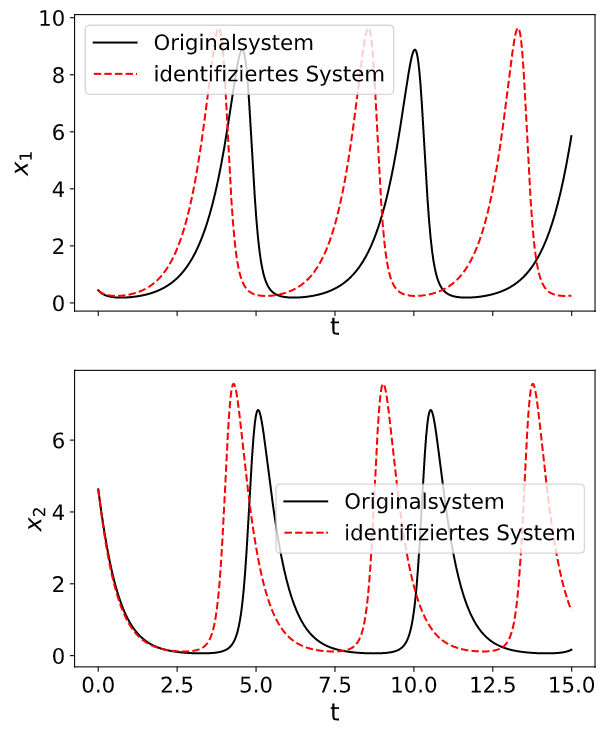
\includegraphics[width=75mm]{images/sim_volterra_e_0_1_sim.png}
	  \caption{Simulationsverlauf}
	  \label{fig:sim_volterra_e_0.1_sim}
	\end{subfigure}%
	\begin{subfigure}{.5\textwidth}
	  \centering
	  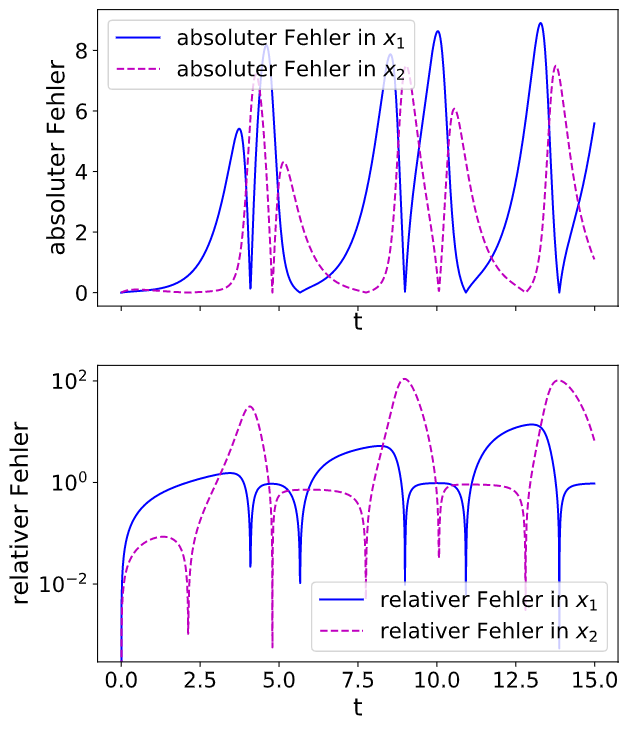
\includegraphics[width=75mm]{images/sim_volterra_e_0_1_err.png}
	  \caption{Fehlerverlauf}
	  \label{fig:sim_volterra_e_0.1_err}
	\end{subfigure}
	\caption{Simulation des Lotka-Volterra-Systems, relativer Fehler der identifizierten Koeffizienten $\varepsilon_\text{r} = 10 \%. $ }
	\label{fig:sim_volterra_e_0.1}
\end{figure}
\begin{figure}[h] %sim
	\centering
	\begin{subfigure}{.5\textwidth}
	  \centering
	  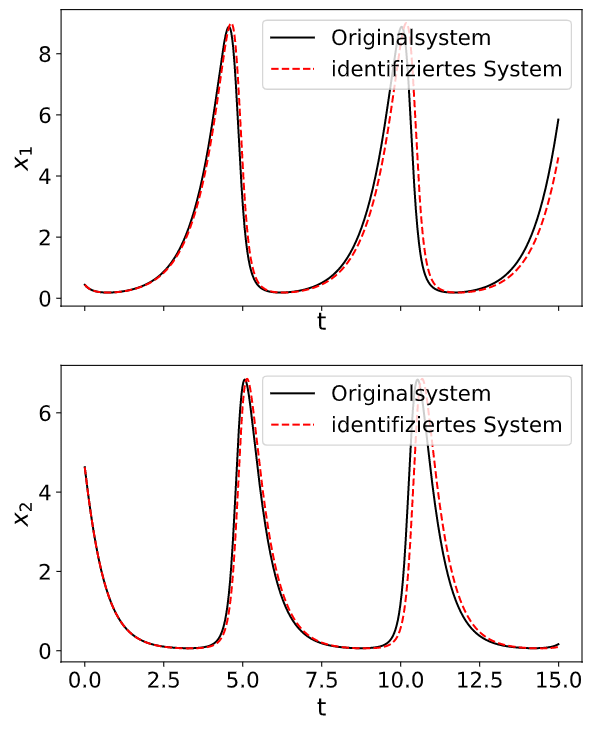
\includegraphics[width=75mm]{images/sim_volterra_e_0_01_sim.png}
	  \caption{Simulationsverlauf}
	  \label{fig:sim_volterra_e_0.01_sim}
	\end{subfigure}%
	\begin{subfigure}{.5\textwidth}
	  \centering
	  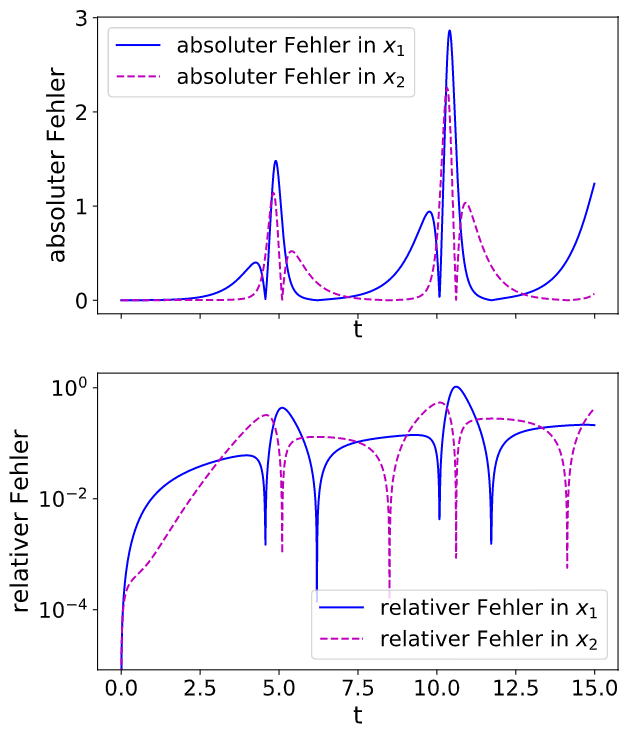
\includegraphics[width=75mm]{images/sim_volterra_e_0_01_err.png}
	  \caption{Fehlerverlauf}
	  \label{fig:sim_volterra_e_0.01_err}
	\end{subfigure}
	\caption{Simulation des Lotka-Volterra-Systems, relativer Fehler der identifizierten Koeffizienten $\varepsilon_\text{r} = 1 \%. $ }
	\label{fig:sim_volterra_e_0.01}
\end{figure}
\begin{figure}[h] %sim
	\centering
	\begin{subfigure}{.5\textwidth}
	  \centering
	  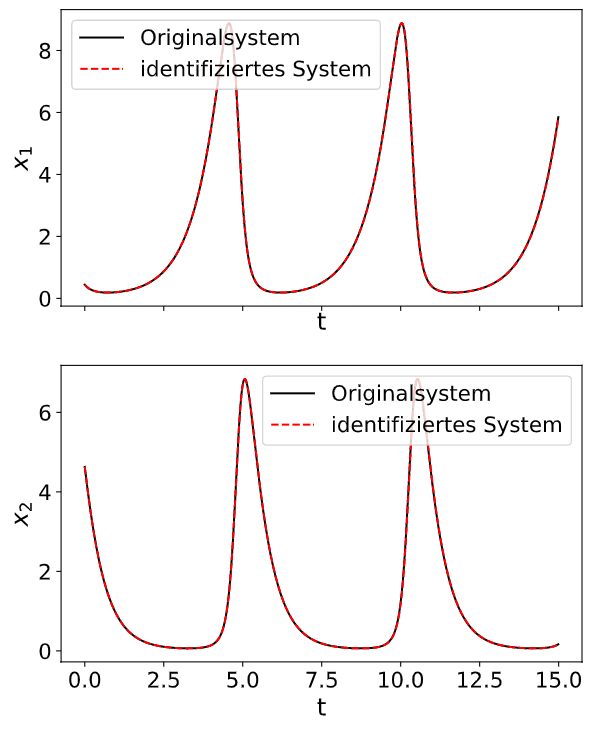
\includegraphics[width=75mm]{images/sim_volterra_e_0_001_sim.png}
	  \caption{Simulationsverlauf}
	  \label{fig:sim_volterra_e_0.001_sim}
	\end{subfigure}%
	\begin{subfigure}{.5\textwidth}
	  \centering
	  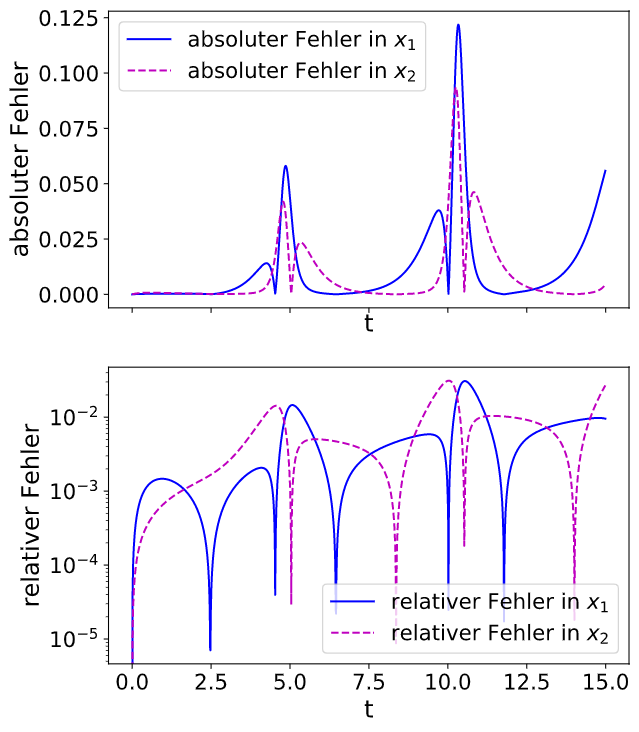
\includegraphics[width=75mm]{images/sim_volterra_e_0_001_err.png}
	  \caption{Fehlerverlauf}
	  \label{fig:sim_volterra_e_0.001_err}
	\end{subfigure}
	\caption{Simulation des Lotka-Volterra-Systems, relativer Fehler der identifizierten Koeffizienten $\varepsilon_\text{r} = 0.1 \%.  $ }
	\label{fig:sim_volterra_e_0.001}
\end{figure}

Um die nachfolgend gezeigten Fehler in den identifizierten Koeffizienten in Relation setzen zu können, ist es sinnvoll, einen Blick auf Simulationen der identifizierten Systeme zu werfen. Abb. \ref{fig:sim_volterra_e_0.1},  \ref{fig:sim_volterra_e_0.01} und \ref{fig:sim_volterra_e_0.001} zeigen die Simulation des Lotka-Volterra-Systems mit unterschiedlich gut identifizierten Koeffizienten. Je kleiner der relative Fehler $\varepsilon_r$ der Koeffizienten ist, desto länger kann das identifizierte System als gute Näherung für das Originalsystem genutzt werden. Wie lange dies der Fall sein soll ist im Einzelfall von der gegebenen Anwendung abhängig und gibt damit auch eine Vorgabe für den maximal erlaubten Fehler der identifizierten Koeffizienten. Im Folgenden wird ein Identifikationsfehler $\varepsilon_\text{r}$ als klein und damit die Identifikation als erfolgreich befunden, wenn $\varepsilon_\text{r} < 1\%$. 

Der relative Fehler der Nominalableitungen zeigt den geringstmöglichen Fehler, den die Methode theoretisch erzielen könnte, wenn die Messungen der Zustandsableitungen exakt wären. Ist dieser Fehler null, so ist unter den gegebenen Parametern eine Systemidentifikation prinzipiell möglich. Im Praxisfall ist der Erfolg der Identifikation jedoch weiterhin von einem geeigneten Zusammenspiel zwischen Algorithmus-Parametern und den Messfehlern in den Datenreihen abhängig. Ist der Fehler bereits im Nominalfall nicht klein genug, so ist eine Identifikation bei Verwendung der Zentraldifferenz nicht möglich. Das deutet darauf hin, dass die Algorithmus-Parameter ungünstig gewählt sind.




Es wird der Einfluss der nachfolgenden Parameter auf das Identifikationsergebnis untersucht. Für die Untersuchung werden Standardwerte festgelegt, die konstant bleiben, während der zu untersuchende Parameter verändert wird. Diese werden in eckigen Klammer angegeben.
\begin{itemize}
\item die Simulationszeit $t$ des DGL-Lösers, [3s],
\item die Schrittweite $dt$ des DGL-Lösers, [0.01s], 
%\item die Anzahl der gleichzeitig analysierten Datenreihen, [eine Datenreihe],
\item die Gestaltung der Bibliothek von Ansatzfunktionen, [Polynome maximal zweiter Ordnung],
%\item das verwendete Optimierungsverfahren zur Lösung des Approximationsproblems, [rekursive MKQ]
\item die Stärke des Rauschens in den Daten, [kein Rauschen].
\end{itemize}
Die Standardparameter sind so gewählt, dass der resultierende Fehler für alle Systeme bereits klein ist. Die Veränderung eines Parameters kann dann den Bereich zeigen, in dem dieser noch sinnvoll verändert werden kann.

\subsection{Einfluss der Simulationszeit}
Wie aus Abb. \ref{fig:errors_tspan} hervorgeht, sinkt der relative Fehler der identifizierten Parameter bei Verwendung der Zentraldifferenz mit steigender Simulationszeit. Dabei ist auffällig, dass für zu geringe Simulationszeiten keine Systemidentifikation möglich ist, während sich der Fehler ab einer gewissen Mindestsimulationszeit kaum noch verändert. Diese Mindestzeit ist notwendig, damit charakteristische Zustandsverläufe sichtbar werden, ähnlich wie die Sinusfunktion mit der Winkelhalbierenden verwechselt werden kann, wenn das Betrachtungsfenter ungünstig gewählt wird. Allerdings sinkt der Fehler für große Simulationszeiten nicht mehr signifikant. Damit existiert für jedes System eine optimale Simulationsdauer.
\begin{figure} %errors tspan
	\centering
%	\begin{subfigure}{.5\textwidth}
%	  \centering
%	  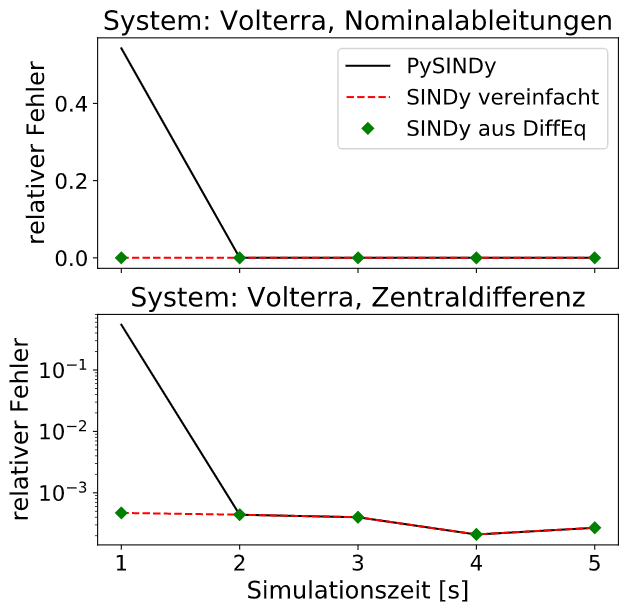
\includegraphics[width=75mm]{images/errors_volterra_tspan_variation.png}
%	  \caption{Lotka-Volterra-System}
%	  \label{fig:errors_volterra_tspan}
%	\end{subfigure}%
%	\begin{subfigure}{.5\textwidth}
%	  \centering
	  \includegraphics[width=75mm]{images/errors_roessler_tspan_variation.png}
%	  \caption{Rössler-System}
%	  \label{fig:errors_roessler_tspan}
%	\end{subfigure}
	\caption{relativer Fehler der identifizierten Parameter in Abhängigkeit der Simulationszeit.}
	\label{fig:errors_tspan}
\end{figure}

\subsection{Einfluss der Simulationsschrittweite}
Um Anforderungen an die Messung der Zustandskomponenten zu minimieren, ist es sinnvoll zu fordern, dass die Zeit zwischen zwei Messungen (hier durch die Simulationsschrittweite repräsentiert) so groß wie möglich gewählt wird. In Abb. \ref{fig:errors_dt} zeigt sich, dass der Fehler mit zunehmender Schrittweite steigt. Jedes System besitzt eine spezifische Schrittweite, ab welcher keine Identifikation mehr möglich ist. Anders als bei der Simulationszeit sinkt der Fehler hier für kleine Schrittweiten immer weiter, bis hin zum Extremfall, dass die Schrittweite infinitesimal klein ist und der Fehler null wird (siehe Nominalfall). Damit muss man bei der Auswahl der Schrittweite zwischen Genauigkeit und Messaufwand abwägen.
\begin{figure} %errors dt
	\centering
	\begin{subfigure}{.5\textwidth}
	  \centering
	  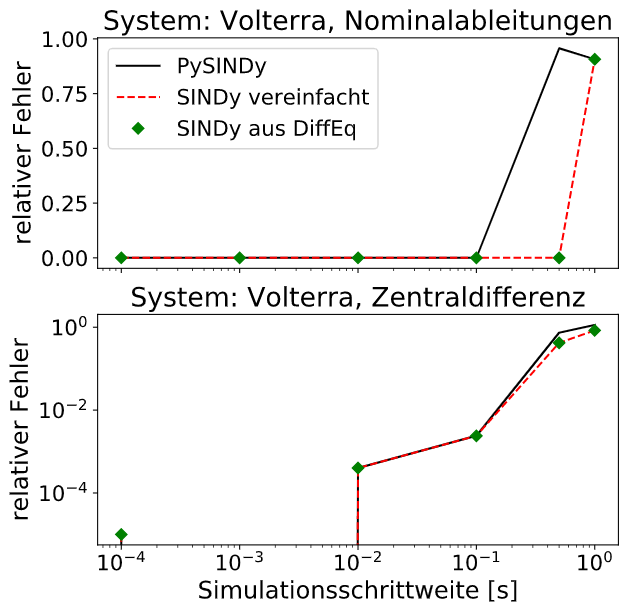
\includegraphics[width=75mm]{images/errors_volterra_dt_variation.png}
	  \caption{Lotka-Volterra-System}
	  \label{fig:errors_volterra_dt}
	\end{subfigure}%
	\begin{subfigure}{.5\textwidth}
	  \centering
	  \includegraphics[width=75mm]{images/errors_lorenz_dt_variation.png}
	  \caption{Lorenz-System}
	  \label{fig:errors_lorenz_dt}
	\end{subfigure}
	\caption{relativer Fehler der identifizierten Parameter in Abhängigkeit der Simulationsschrittweite.}
	\label{fig:errors_dt}
\end{figure}

\subsection{Einfluss der Gestaltung der Bibliothek}
Wie bereits angedeutet ist die Auslegung der Bibliothek entscheidend für eine erfolgreiche Identifikation. Je weniger Informationen dem Algorithmus im Vorhinein zur Verfügung gestellt werden müssen, desto mächtiger ist er. Daher ist es wünschenswert, die Bibliothek so groß wie möglich ansetzen zu können, um auch Funktionsklassen zu beinhalten, deren Vorkommen nicht gesichert ist. Für die drei zu untersuchenden Systeme wurde eine polynomiale Bibliothek angesetzt, die schrittweise durch Monome höherer Ordnung ergänzt wurde. Abb. \ref{fig:errors_order} zeigt, dass die Bibliothek mit deutlich mehr Funktionen besetzt werden kann als nötig und eine Identifikation trotzdem noch möglich ist. Allerdings gibt es auch hier einen Punkt, ab dem die Identifikation scheitert. Mit zunehmender Anzahl an Funktionen wird es wahrscheinlicher, dass eine Linearkombination dieser Funktionen existiert, die eine in der DGL vorkommende Funktion hinreichend genau beschreibt und ein Teil des Ergebnisses wird. Die so entstandene DGL kann das System in der Regel ausreichend gut numerisch modellieren, ist aber auf Grund der falsch identifizierten Ansatzfunktionen nur als Black-Box-Modell zu gebrauchen und für die Identifikation von analytischen Zusammenhängen unbrauchbar.

\begin{figure}[h!] %errors order
	\centering
	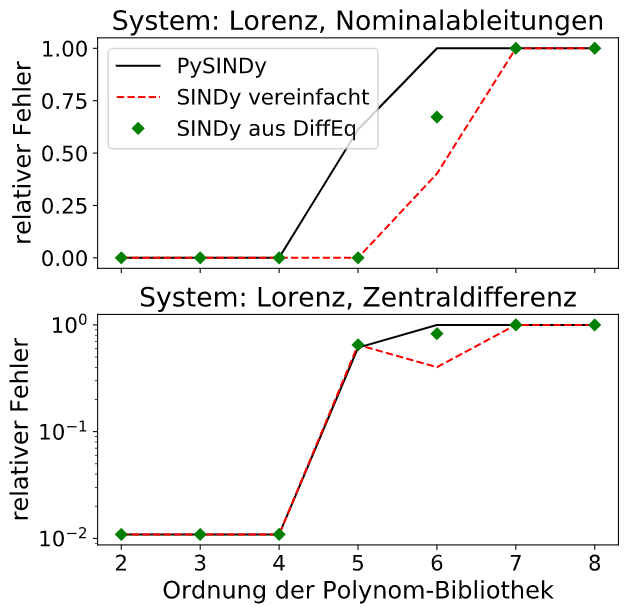
\includegraphics[width=75mm]{images/errors_Lorenz_order_variation.png}
	\caption{relativer Fehler der Identifizierten Parameter in Abhängigkeit der Ordnung der Polynom-Bibliothek.}
	\label{fig:errors_order}
\end{figure}

\subsection{Einfluss von verrauschten Daten}
Für die folgende Untersuchung (Abb. \ref{fig:errors_noise}) wurden die Verläufe der Zustandskomponenten mit additivem weißen Rauschen überlagert. Die Stärke des Rauschsignals wurde über die Standardabweichung der verwendeten Normalverteilung eingestellt. Je stärker das Rauschen, desto ungenauer werden die identifizierten Koeffizienten. Wie stark verrauscht die Daten sein können, sodass dennoch eine Identifikation möglich ist, hängt vom System ab.
\begin{figure}[h!] %errors noise
	\centering
	\begin{subfigure}{.5\textwidth}
	  \centering
	  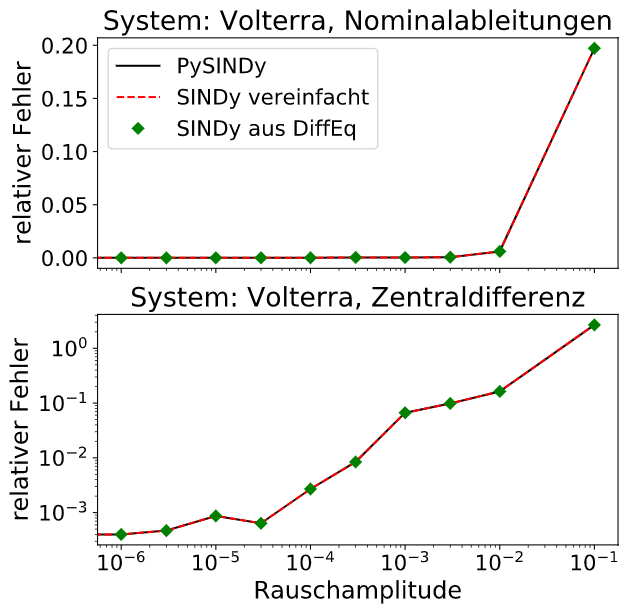
\includegraphics[width=75mm]{images/errors_volterra_noise_variation.png}
	  \caption{Lotka-Volterra-System}
	  \label{fig:errors_volterra_noise}
	\end{subfigure}%
	\begin{subfigure}{.5\textwidth}
	  \centering
	  \includegraphics[width=75mm]{images/errors_lorenz_noise_variation.png}
	  \caption{Lorenz-System}
	  \label{fig:errors_lorenz_noise}
	\end{subfigure}
	\caption{relativer Fehler der identifizierten Parameter in Abhängigkeit der Rauschstärke.}
	\label{fig:errors_noise}
\end{figure}

\subsection{Rechenzeit}
Abb. \ref{fig:time} zeigt exemplarisch das qualitative Verhältnis der Rechenzeiten der Implementationen. Beide \textit{Python}-Implementationen sind deutlich schneller als die \textit{Julia}-Version. Dennoch ist die Rechenzeit in allen Fällen recht klein. Der vereinfachte Algorithmus schneidet am besten ab, was damit zu erklären ist, dass viele periphere Funktionen, wie die Validierung der Eingabedaten, nicht implementiert sind.

\begin{figure}[h!] %times
	\centering
	\begin{subfigure}{.5\textwidth}
	  \centering
	  
\includegraphics[width=75mm]{images/time_volterra_dt.png}
	  %\caption{Lotka-Volterra-System}
	%  \label{fig:time_volterra_dt}
	\end{subfigure}%
	\begin{subfigure}{.5\textwidth}
	  \centering
	  
\includegraphics[width=75mm]{images/time_roessler_noise.png}
	  %\caption{Roessler-System}
	 % \label{fig:time_roessler_noise}
	\end{subfigure}
	\caption{durchschnittliche Rechenzeit der unterschiedlichen Algorithmen.}
	\label{fig:time}
\end{figure}


\subsection{Zusammenfassung der Ergebnisse}
Anders als zu Beginn der Arbeit vermutet, lassen sich keine Unterschiede in der Genauigkeit der SINDy-Implementationen feststellen. Allerdings ist die richtige Wahl der Parameter von großer Bedeutung für die Qualität der Identifikation. Die identifizierten Parameter werden genauer, wenn mehr Messdaten zur Verfügung stehen, also die Anzahl der Messungen steigt und der zeitliche Abstand zwischen ihnen verringert wird. Der Algorithmus kann mit verrauschten Messdaten arbeiten, genauere Messungen liefern bessere Ergebnisse. Die Bibliothek aus Ansatzfunktionen muss groß genug sein, um alle in den Systemgleichungen vorkommenden Ansatzfunktionen zu beinhalten und gleichzeitig klein genug, damit die Richtigen ausgewählt werden. Leider sind die optimalen Parameter von System zu System unterschiedlich, sodass hier keine allgemeingültigen Aussagen zur Größe von Parametern getroffen werden können.


\section{Verbesserung der Ergebnisse}
\subsection{Arbeit mit mehreren Trajektorien}
Wenn die Identifikation in den bisher betrachteten Beispielen scheiterte, dann wurde statt der korrekten rechten Seite einer Differentialgleichung eine andere Linearkombination von Ansatzfunktionen identifiziert, die einen kleineren Fehler \eqref{eq:Fehler_MKQ} hinterlässt und das System somit ''besser'' modelliert. Anschaulich bedeutet das, dass aus den genutzten Daten die Dynamik des Systems nicht eindeutig herauszulesen war. Dabei spielen die Anfangswerte der verwendeten Trajektorie eine entscheidende Rolle. Besitzt das System beispielsweise eine Ruhelage und wird diese als Anfangswert dem Differentialgleichungslöser vorgegeben, so ist aus der resultierenden Trajektorie keine Systemidentifikation möglich. Daher kann es nützlich sein, mehrere Trajektorien mit verschiedenen Anfangswerten zu verwenden. Umgesetzt wird dies, indem die Matrizen der Zustands- und Ableitungsverläufe untereinander angeordnet werden
\begin{equation}
X = \begin{bmatrix}
		X_1 \\
		X_2 \\
		\vdots   \\ 
		X_t
	\end{bmatrix} \in \mathbb{R}^{m\cdot t\times n},\quad
	\dot{X} = \begin{bmatrix}
			\dot{X}_1 \\
			\dot{X}_2 \\
			\vdots   \\ 
			\dot{X}_t
		\end{bmatrix} \in \mathbb{R}^{m\cdot t\times n}.
\end{equation}
In Abb. \ref{fig:errors_no_tr} wurde jeder Parameter so ungünstig gewählt, dass allein dieser die Identifikation schwierig machen würde (Simulationszeit von 1s, Schrittweite von 0.1s, Bibliothek aus Polynomen bis zur Ordnung 5, Weißes Rauschen mit Standardabweichung von $10^{-4}$). Durch die Verwendung von ausreichend vielen Messreihen kann die Identifikation dennoch gelingen.
\begin{figure}[h!] %errors no_tr
	\centering
	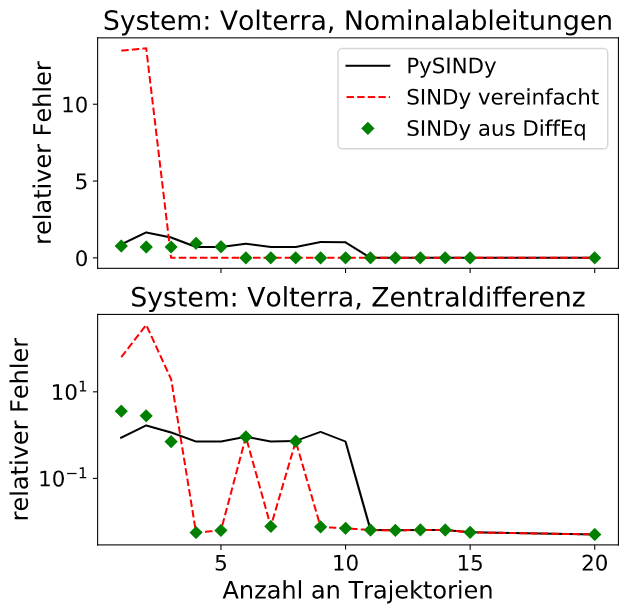
\includegraphics[width=75mm]{images/errors_volterra_no_tr_variation2.png}
	\caption{relativer Fehler der identifizierten Parameter in Abhängigkeit der Anzahl der gleichzeitig verwendeten Trajektorien.}
	\label{fig:errors_no_tr}
\end{figure}
\subsection{Identifikation von teilweise bekannten Systemen}
Rackauckas et al. \cite{Rackauckas2020} zeigen, wie man Wissen über bereits bekannte Teilsysteme in die Identifikation integrieren kann. Angenommen man möchte das Lotka-Volterra-System \eqref{eq:volterra} identifizieren und kennt bereits die linearen Terme und ihre Koeffizienten. Dann lässt sich das System darstellen als
\begin{equation}
	\begin{aligned}
		\dot{x} &= \alpha x + U_1(x,y)\\
		\dot{y} &= \gamma y + U_2(x,y),
	\end{aligned}
\end{equation}
mit den unbekannten nichtlinearen Termen $U_1(x,y)$ und $U_2(x,y)$. Da die Zustandsableitungen als bekannt angenommen werden (durch Messung oder Zentraldifferenz aus den Zuständen ermittelt), können die unbekannten Terme auf der rechten Seite isoliert werden:
\begin{equation}
	\begin{aligned}
		\dot{x} - \alpha x &= U_1(x,y)\\
		\dot{y} - \gamma y &= U_2(x,y).
	\end{aligned}
\end{equation}
Somit kann die angepasste linke Seite der Differentialgleichung folgendermaßen konstruiert werden:
\begin{equation}
\dot{X} = \begin{bmatrix} 
		\dot{x}(t_1)-\alpha x(t_1) & \dot{y}(t_1)-\gamma y(t_1) \\
		\dot{x}(t_2)-\alpha x(t_2) & \dot{y}(t_2)-\gamma y(t_2) \\
		\vdots 		   & \vdots 	 \\
		\dot{x}(t_m)-\alpha x(t_m) & \dot{y}(t_m)-\gamma y(t_m) \\
	\end{bmatrix}  \in \mathbb{R}^{m\times 2}.
\end{equation}
Von hier aus kann der Algorithmus wie bekannt weiterlaufen. 

Eine Voraussetzung für diese Methode ist, dass sich bekannte und unbekannte Teilsysteme voneinander isolieren lassen. Dies ist der Fall, wenn eine bekannte Funktion $K(\boldsymbol{x})\in\mathbb{R}^{n}$ und eine unbekannte Funktion $U(\boldsymbol{x})\in\mathbb{R}^{n}$ existieren, sodass die Umformung
\begin{equation}
 K(\boldsymbol{x}) \circ \dot{\boldsymbol{x}} = U(\boldsymbol{x})
\end{equation} 
möglich ist. Ist dies nicht der Fall, z.B. für
\begin{equation}
\dot{\boldsymbol{x}} = K_1(\boldsymbol{x})\cdot U_1(\boldsymbol{x}) + K_2(\boldsymbol{x})\cdot U_2(\boldsymbol{x}),
\end{equation}
dann kann das Wissen über das bekannte Teilsystem nur in die Gestaltung der Bibliothek einfließen, nicht jedoch die Identifikation wie beschrieben von Anfang an vereinfachen.
Dieses Problem wird in Abschnitt \ref{sec:aufbauderbibo} noch einmal aufgegriffen.










\chapter{Anwendung auf komplexes Beispiel - Inverses Pendel}
\section{Einleitung}
Ein beliebtes regelungstechnisches Problem ist die Regelung eines inversen Pendels an einem Wagen (Abb. \ref{fig:wp}). Die Voraussetzung dafür ist das Vorhandensein eines guten Systemmodells. Während solche Modelle berechnet werden können \cite[Softwarebeispiel 3]{Knoll2016}, soll hier untersucht werden, ob ähnliche Ergebnisse mit SINDy reproduziert werden können, oder ob SINDy zur Parameterschätzung genutzt werden kann. 
\begin{figure}[h!] %wp
	\centering
	\includegraphics[width=75mm]{images/wp.jpg}
	\caption{Schematische Darstellung des Wagen-Pendel-Systems, mit den Massen $m_1$ und $m_2$, der Pendellänge $s$, der Erdbeschleunigung $g$, dem Krafteingang $F$, der Position des Wagens $x$ und der Auslenkung des Pendels aus der unteren Ruhelage $\varphi$.}
	\label{fig:wp}
\end{figure}
Das Wagen-Pendel-System wird durch folgende DGL beschrieben:
\begin{align}
	\dot{\boldsymbol{x}} &= \begin{pmatrix}
		\dot{x_1}  \\
		\dot{x_2}  \\
		\dot{x_3}  \\ 
		\dot{x_4}	
	\end{pmatrix} 	=	\begin{pmatrix}
							\dot{\varphi} \\
							\dot{x}  \\
							\ddot{\varphi}  \\ 
							\ddot{x}
						\end{pmatrix} = f(\boldsymbol{x}) + g(\boldsymbol{x}) u\\
	&=\begin{pmatrix}
		\dot{\varphi}  \\
		\dot{x}  \\
		-\frac{m_2s\dot{\varphi}^2\sin\varphi\cos\varphi + (m_1+m_2)g\sin\varphi}{s(m_1 + m_2\sin^2\varphi)}\\
		\frac{gm_2\sin\varphi\cos\varphi + m_2s\dot{\varphi}^2\sin\varphi}{(m_1+m_2\sin^2\varphi)}   
	\end{pmatrix}		
 +		 \begin{pmatrix}
									0  \\
									0  \\
									-\frac{\cos\varphi}{s(m_1 + m_2\sin^2\varphi)}\\
									\frac{1}{m_1+m_2\sin^2\varphi}   
								\end{pmatrix} F. \label{eq:wp}
\end{align}
Der Einfachheit halber wird nur das autonome System betrachtet, daher gilt $F\equiv0$. 
Ausgehend von den zeitlichen Verläufen der Zustandskomponenten und deren Ableitungen sollen die Struktur und die Parameter $\boldsymbol{p}=\begin{pmatrix*}[c] m_1& m_2& s & g \end{pmatrix*}$ des Systems bestimmt werden.

\section{Aufbau der Bibliothek}
\label{sec:aufbauderbibo}
Das Wagen-Pendel-System wird im Gegensatz zu den bisher betrachteten Systemen nicht ausschließlich durch Polynome beschrieben. Das macht die Konstruktion der Bibliothek deutlich schwieriger. Der Algorithmus berechnet eine Linearkombination von Ansatzfunktionen, die das System modellieren sollen. Schreibt man die letzten beiden Zeilen von \eqref{eq:wp} als Summe
\begin{equation}
	\begin{pmatrix}
		\ddot{\varphi}  \\
		\ddot{x}  	
	\end{pmatrix}
	=\begin{pmatrix}
		-\frac{m_2s\dot{\varphi}^2\sin\varphi\cos\varphi}{sm_1 + sm_2\sin^2\varphi} - \frac{(m_1+m_2)g\sin\varphi}{sm_1 + sm_2\sin^2\varphi}\\
		\frac{gm_2\sin\varphi\cos\varphi}{m_1+m_2\sin^2\varphi} + \frac{m_2s\dot{\varphi}^2\sin\varphi}{m_1+m_2\sin^2\varphi}  , 
	\end{pmatrix}		
\end{equation}
so fällt auf, dass in jeder Zeile nur zwei verschiedene Ansatzfunktionen vorkommen. Diese müssen dem Algorithmus in der Bibliothek vorgegeben werden. Es lohnt sich darauf hinzuweisen, dass es nicht ausreicht, eine Bibliothek aus den vorkommenden Elementarfunktionen ($\sin, \cos$, Zustandskomponenten, Identität) anzulegen in der Hoffnung, dass SINDy diese geeignet verknüpft. SINDy kann die vorgegeben Funktionen nur additiv durch die angesprochene Linearkombination verknüpfen. 
Damit eine Identifikation möglich ist, muss sich jede Zeile der DGL wie folgt aus Funktionen $u_i$ und $v_i$ darstellen lassen:
\begin{equation}
x_i=\sum_{k}u_k(\boldsymbol{p})v_k(\boldsymbol{x}), \label{eq:right_side_decomp}
\end{equation}
wobei $u_i$ nicht von $\boldsymbol{x}$ und $v_i$ nicht von $\boldsymbol{p}$ abhängig sein darf. Dies ist auf Grund der Struktur der Nenner hier nicht möglich. Daher müssen die Nenner in diesem Beispiel als bekannt vorausgesetzt werden. 
Die Zähler haben eine für die Identifikation günstige Struktur, da sie Bedingung \eqref{eq:right_side_decomp} erfüllen. Dabei werden maximal vier Elementarfunktionen miteinander multipliziert. Um die Bibliothek systematisch aufzubauen, müssten für die Zähler alle Kombinationen mit Wiederholung aus maximal vier Elementarfunktionen berücksichtigt werden. Damit ergeben sich $C^r(13,4) = 1820$\footnote{Es gibt 13 mögliche Faktoren: $\sin$ und $\cos$ von jeder Zustandskomponente, vier Zustandskomponenten, Identität.} mögliche Zähler, wodurch die Bibliothek viel zu groß ist. Um das zu verhindern müssen einschränkende Annahmen getroffen werden:
\begin{itemize}
\item Nur die Auslenkung des Pendels aus der unteren Ruhelage $\varphi$ darf als Argument der Winkelfunktionen verwendet werden. 
\item Nur $\dot{\varphi}$ kann außerhalb der Winkelfunktionen vorkommen.
\end{itemize}
Damit verringert sich die Anzahl an möglichen Zählern auf $C^r(4,4) = 35$. Aus diesen Zählern und den bekannten Nennern kann der Großteil der Ansatzfunktionen für die Bibliothek erzeugt werden. Es fehlen nur noch Monome ersten Grades, um die ersten beiden Zeilen der DGL abbilden zu können. Damit ergibt sich eine Bibliothek aus 39 Ansatzfunktionen. Jedoch liefert diese noch nicht das gewünschte Ergebnis. Problematisch ist, dass es in der Bibliothek linear abhängige Spalten gibt, da gilt: 
\begin{equation}
\cos \varphi = \cos ^3 \varphi+ \sin^2 \varphi\cos \varphi.
\end{equation}
Dadurch kann, statt der vollständig vereinfachten Gleichung, eine zwar mathematisch richtige, jedoch wenig verwertbare Gleichung geliefert werden, da diese erst vereinfacht und die Koeffizienten neu berechnet werden müssten. Stattdessen kann man die Bibliothek noch einmal verkleinern, indem man die linear abhängigen Spalten entfernt. Diese kann man finden, indem man den Spaltenrang der ersten $i$ Spalten mit dem Spaltenrang der ersten $i+1$ Spalten der Bibliothek vergleicht. Sind die Ränge gleich, ist die $i+1$-te Spalte von den ersten $i$ Spalten linear abhängig und kann entfernt werden. Führt man diesen Prozess für die gesamte Bibliothek aus, so bleiben am Ende noch 28 Ansatzfunktionen übrig\footnote{Die Auswahl der 28 Spalten ist nicht eindeutig, aber mathematisch äquivalent, da die resultierenden Gleichungen gegebenenfalls vereinfacht werden können.}. Die Bibliotheksmatrix besitzt vollen Rang.

\section{Bewertung der Ergebnisse}
Unter Nutzung des Wissens über die geeignete Wahl der Identifikationsparameter und Verwendung mehrerer Trajektorien ist die Identifikation, wie in Abb. \ref{fig:sim_wp} ersichtlich, erfolgreich.
\begin{figure}[h!] %sim
	\centering
	\begin{subfigure}{.5\textwidth}
	  \centering
	  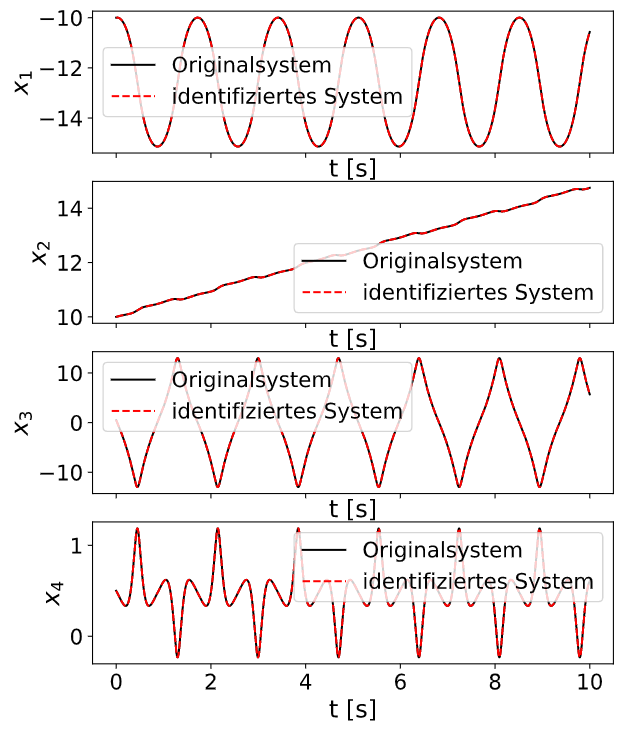
\includegraphics[width=75mm]{images/sim_wp_sim.png}
	  \caption{Simulationsverlauf}
	  \label{fig:sim_wp_sim}
	\end{subfigure}%
	\begin{subfigure}{.5\textwidth}
	  \centering
	  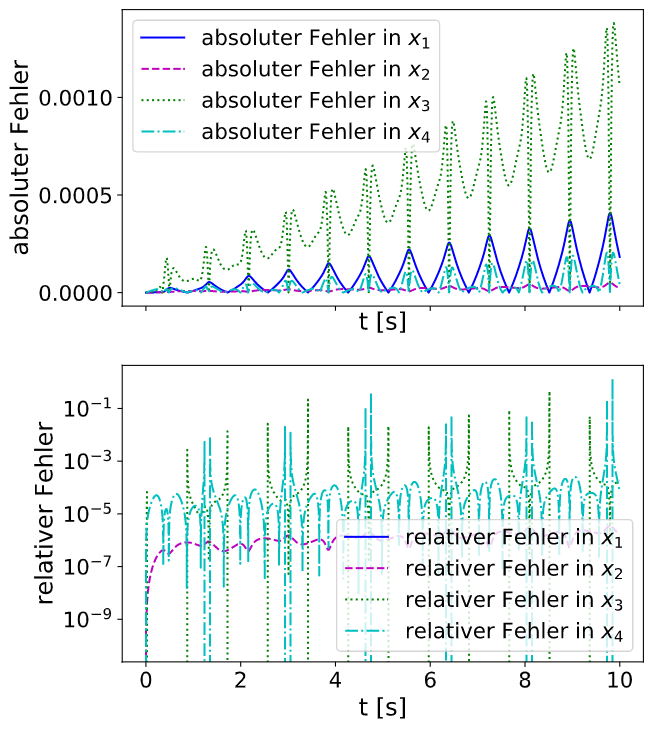
\includegraphics[width=75mm]{images/sim_wp_err.png}
	  \caption{Fehlerverlauf}
	  \label{fig:sim_wp_err}
	\end{subfigure}
	\caption{Simulation des Wagen-Pendel-Systems, relativer Fehler der identifizierten Koeffizienten $\varepsilon_\text{r} = 8\cdot 10^{-5}$.}
	\label{fig:sim_wp}
\end{figure}
Auf Grund der komplexen Struktur des Wagen-Pendel-Systems ist der SINDy-Algorithmus ohne beträchtliches Vorwissen über das System und einige Vereinfachungen nicht geeignet. Lassen sich die Differentialgleichungen nicht als Linearkombination relativ einfacher Funktionen darstellen, stößt die Methode schnell an ihre Grenzen. Allerdings zeigt das Beispiel, dass SINDy sehr gute Ergebnisse liefern kann, wenn die Struktur des Systems bereits bekannt ist und nur Parameter geschätzt werden sollen. 








\chapter{Zusammenfassung und Ausblick}
\section{Zusammenfassung}
In dieser Arbeit wurde der SINDy-Algorithmus als Methode zur Gewinnung von Systemdifferentialgleichungen aus Messdaten untersucht. Es wurde der Einfluss verschiedener Parameter auf das Identifikationsergebnis vorgestellt und Richtlinien zu deren Einstellung abgeleitet. SINDy ist besonders für die Identifikation parameterlinearer Systeme geeignet, darüber hinaus muss man viel Vorwissen beisteuern, um brauchbare Ergebnisse zu erzielen. Allgemein ist das benötigte Vorwissen über das zu untersuchende System ein entscheidender Nachteil der Methode. Ist dieses jedoch vorhanden, so kann SINDy sehr genaue Ergebnisse liefern, was z.B. die Schätzung von Systemparametern angeht.

\section{Ausblick}
Potential für weitere Untersuchungen bietet der SINDy-Algorithmus bei der Identifikation teilweise bekannter Systeme. Oft sind die physikalischen Zusammenhänge eines Systems theoretisch bekannt. SINDy kann dann dazu genutzt werden, nur parasitäre Einflüsse wie Reibungen zu modellieren. 
Eine weitere vorstellbare Anwendung könnte die Echtzeitschätzung von Parametern sein. Die Messdaten der Zustandskomponenten werden zur Laufzeit, z.B. durch einen Beobachter, gesammelt und mittels SINDy werden die Systemparameter aktualisiert. 


%\csvautotabular{images/errors_volterra_tspan_variation.csv} 





%
%
%
%\chapter{Notizen}
%inhaltlich noch zu verarbeitende Punkte: 
%identification with prior knowledge
%reibung
%rauschen
%vergleichsparameter: tspan, dt, u0, (lambda), multra, p?, order
%NN
%
%ausblick: online systemschätzung
%
%verwendete Parameter:
%default: \\
%dt =0.01\\
%tspan = 3s\\
%opt = LSTSQ/STRRidge\\
%notr = 1\\
%poly order = 2\\
%lambda = 0.2/0.05\\
%u0 = [0.44249296,4.6280594], [-8, 8, 27], [1, -1, -1]\\
%noise = 0\\
%
%no tr variation:
%volterra: dt= 0.1, tspan = 3s
%lorenz: dt = 0.01, tspan = 0.25s
%roessler dt = 0.01, tspan = 0.1s
%
%\section{UDE}
%
%\begin{figure}[ht]
%\begin{subfigure}[c]{0.5\textwidth}
%\centering
%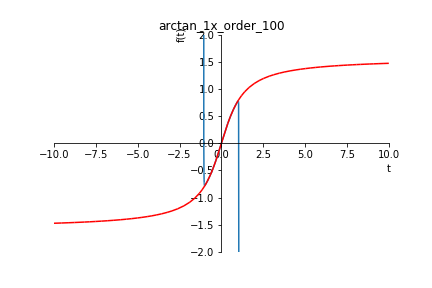
\includegraphics[width=1\textwidth]{images/arctan_1x_order_100}
%
%\end{subfigure}
%\begin{subfigure}[c]{0.5\textwidth}
%\centering
%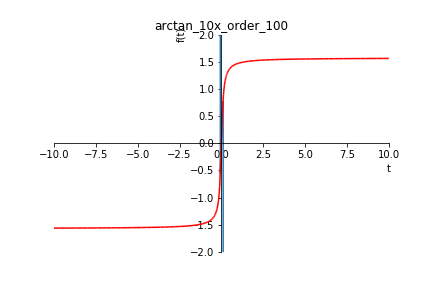
\includegraphics[width=1\textwidth]{images/arctan_10x_order_100}
%
%\end{subfigure}
%\begin{subfigure}[c]{0.5\textwidth}
%\centering
%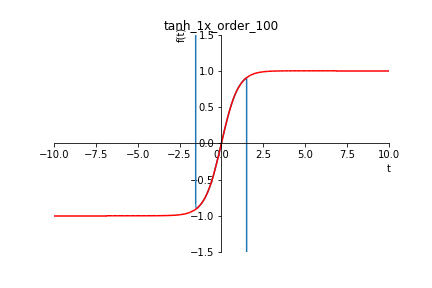
\includegraphics[width=1\textwidth]{images/tanh_1x_order_100}
%
%\end{subfigure}
%\begin{subfigure}[c]{0.5\textwidth}
%\centering
%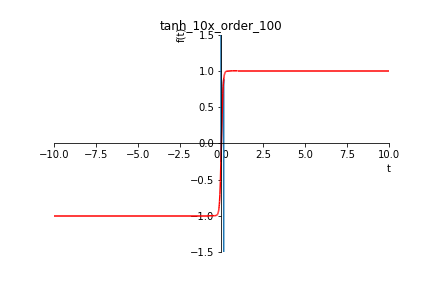
\includegraphics[width=1\textwidth]{images/tanh_10x_order_100}
%
%\end{subfigure}
%\end{figure}
%
%
%\subsection{8.7.20} 
%überlegung NN in julia und sindy in python machen, export erledigt\\
%trotzdem keine identifikation in python möglich, grund: zu wenig daten (datenfeld mit 31 daten Autflösung viel zu gering)\\
%bei erhöhung der auflösung wird trainingszeit enorm groß
%NN approximiert den verlauf der ableitungen	\\
%sindy mal mit anderen anfangswerten trainieren
%\subsection{9.7.20}
%ude keine option für multiple trajectories / threshhold???
%\subsubsection{ude + sindy}
%definitorische Gleichungen bekannt\\
%dt=0.1\\
%sindy did not converge
%\begin{align}
%du_1 &= cos(u_3) * p_1\\
%du_2 &= sin(u_3) * p_2\\
%du_3 &= sin(u_1) * p_3 + p_4 * u_1\\
%du_4 &= sin(u_3) * p_5
%\end{align}
%parameters: Float32[0.050624948, 0.006272168, -20.755184, -13.720979, -0.01513608]
%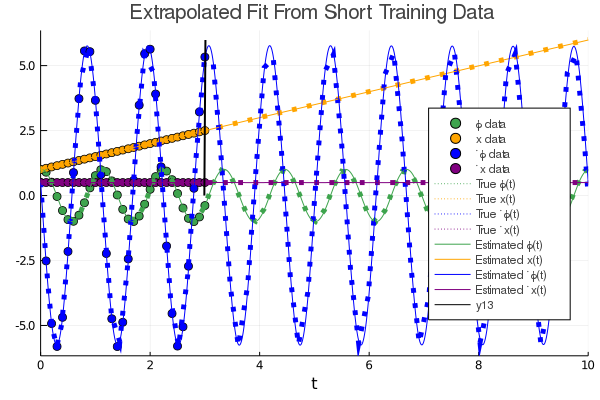
\includegraphics[width=1\textwidth]{images/ude_ident_with_prior_knowledge}
%im Vergleich: nur den Sindy Part in PySindy ausgelagert ergibt: (dieser Vergleich ist nicht sinnvoll? pysindy kennt ja die def. gl nicht)
%\begin{align*}
%phi' &= 65170415.755 xdot + -72812822.138 sin(xdot) + 2647179.524 cos(xdot)\\
%x' &= 51018334.340 xdot + -57002163.483 sin(xdot) + 2072882.755 cos(xdot)\\
%phidot' &= -3.002 phi + -6.328 x + 2682545588.568 xdot + -33.032 sin(phi) \\&+ -1.358 sin(x) + -0.208 sin(phidot) + -2997205703.337 sin(xdot) \\&+ -0.020 cos(phi) + -6.583 cos(x) + 109008747.059 cos(xdot)\\
%xdot' &= 0.320 x + -18300414.600 xdot + 20447317.167 sin(xdot) + 0.344 cos(x) \\&+ -743815.199 cos(xdot)
%\end{align*}
%
%
%
%
%keine Gleichungen bekannt\\
%dt=0.1\\
%sindy did not converge
%\begin{align}
%du_1 &= p_1 * u_3\\
%du_2 &= sin(u_2) * p_2\\
%du_3 &= sin(u_1) * p_3 + p_4 * u_1\\
%du_4 &= cos(u_1) * p_5
%\end{align}
%parameters: Float32[0.997858, 0.20674846, -18.494001, -15.788721, 0.040644586]\\
%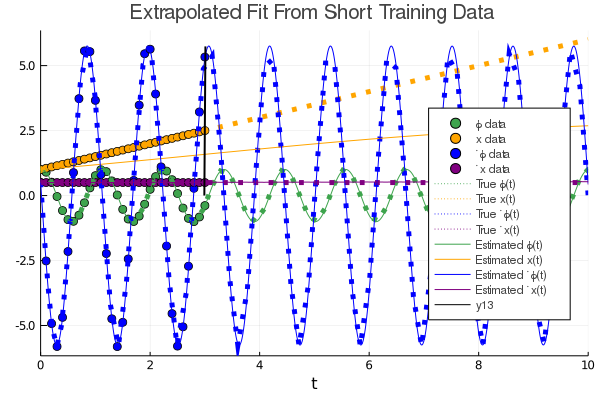
\includegraphics[width=1\textwidth]{images/ude_ident_without_prior_knowledge}
%im Vergleich: nur den Sindy Part in PySindy ausgelagert ergibt:
%\begin{align*}
%phi' &= 1.111 phi + 0.648 x + 1.002 phidot + -503701656.178 xdot + -1.228 sin(phi) \\&+ 562779966.638 sin(xdot) + -0.050 cos(phi) + 0.676 cos(x) + -20465608.922 cos(xdot)\\
%x' &= 0.833 phi + -0.031 x + 450669011.982 xdot + -0.967 sin(phi) \\&+ -503527393.951 sin(xdot) + 0.157 cos(phi) + -0.051 cos(x) + 18310968.307 cos(xdot)\\
%phidot' &= -2.551 phi + -4.834 x + -3252316739.183 xdot + -33.509 sin(phi) \\&+ -0.458 sin(x) + 3633781720.861 sin(xdot) + -5.066 cos(x) + -132146405.440 cos(xdot)\\
%xdot' &= 0.674 phi + -184783222.592 xdot + -0.759 sin(phi) + 206455836.816 sin(xdot) + \\&-7507657.694 cos(xdot)
%\end{align*}
%
%\subsubsection{ude reibung}
%tanh wie erwartet problematisch, vmtl sinnvoll tanh vorzugeben\\
%viskose+ haftreibung:
%\begin{align*}
%du_1 &= sin(u_3) * p_1\\
%du_2 &= cos(u_1) * p_2 + cos(u_3) * p_3\\
%du_3 &= p_4 * u_3\\
%du_4 &= sin(u_3) * p_5
%\end{align*}
%parameters: Float32[-0.032978103, 0.020778582, 0.02180107, -0.30371103, -0.026243187]
%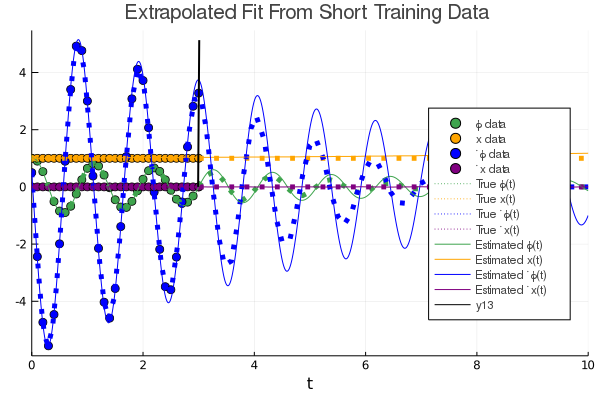
\includegraphics[width=1\textwidth]{images/ude_fric_order_4}
%
%nur viskose reibung, order 2:\\
%\begin{align*}
%d_1&=0.3\\
%d_{1, ident}&= 0.2981498
%\end{align*}
%
%\begin{figure}
%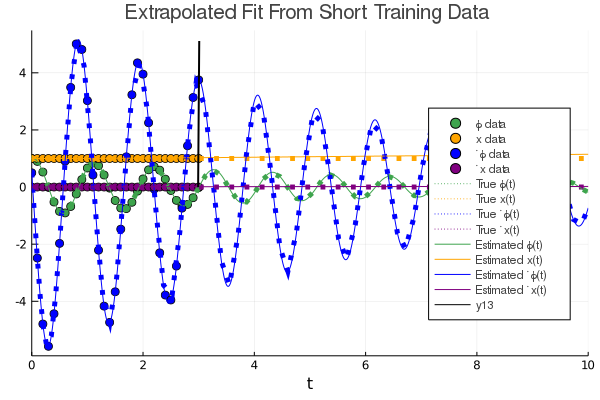
\includegraphics[width=1\textwidth]{images/ude_fric_viskos_d1_03}
%\caption{ude fric viskos d1 03}
%\end{figure}
%
%viskose + haftreibung: order 1, tanh vorgegeben:\\
%\begin{align*}
%du_1 &= cos(u_1) * p_1\\
%du_2 &= sin(u_3) * p_2\\
%du_3 &= tanh(10u_3) * p_3 + p_4 * u_3\\
%du_4 &= tanh(10u_3) * p_5
%\end{align*}
%parameters: Float32[0.018757716, -0.011911368, -0.26272112, -0.35348737, -0.005909097]
%
%\begin{figure}
%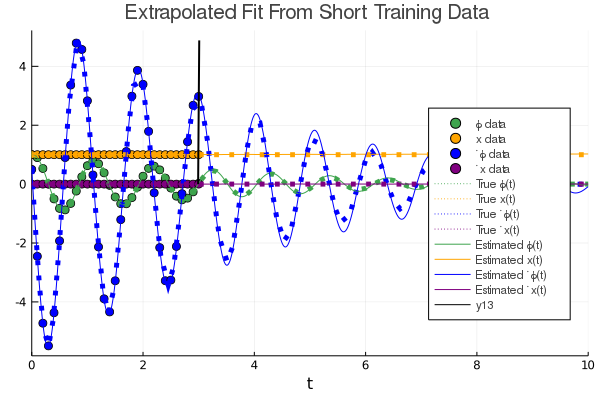
\includegraphics[width=1\textwidth]{images/ude_fric_viskos_d1_03_d2_05}
%\caption{ude fric viskos und haft d1 03 d2 05}
%\end{figure}
%
%
%\subsubsection{Pysindy reibung}
%Ansatz: Sindy für Differenz von Realem Modell mit Reibung und theoretischem Modell verwenden, siehe Bsp:\\
%\begin{figure}
%\begin{subfigure}[c]{0.5\textwidth}
%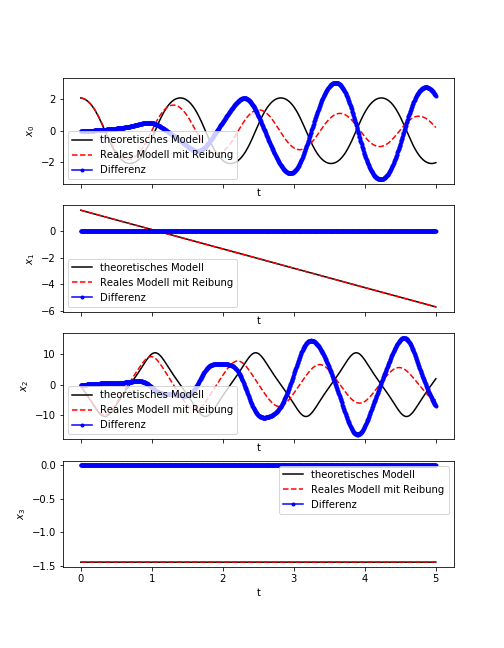
\includegraphics[width=1\textwidth]{images/pysindy_fric_visk2}
%\end{subfigure}
%\begin{subfigure}[c]{0.5\textwidth}
%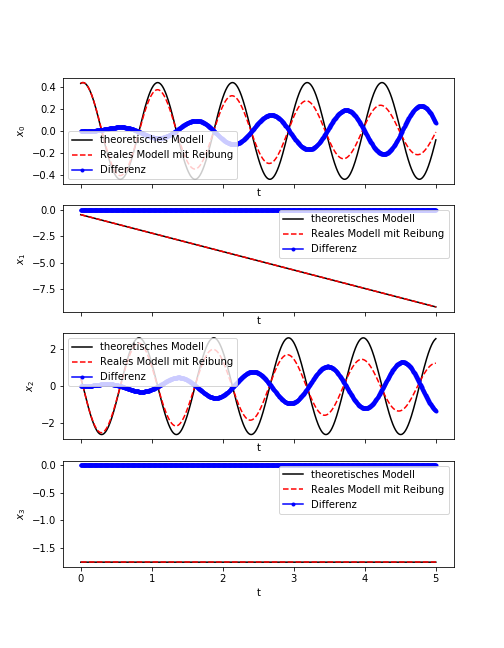
\includegraphics[width=1\textwidth]{images/pysindy_fric_visk1}
%\end{subfigure}
%\caption{nur viskose Reibung}
%\end{figure}
%keine Identifikation feststellbar\\
%vermutung: aus Differenz geht keine exp funktion hervor, es fehlt die info über das vorherige System
%idee: prior system knowledge integrieren indem man das bekannte teilsystem aus library funktion zur verfügung stellt
%\section{Sindy}
%\subsection{Funktionsweise der Methode}
%Sparse Identification of Nonlinear Dynamics (SINDy) ist eine Methode, um aus Messdaten eines Systems dessen Systemdifferentialgleichungen zu schätzen.\\
%Sei $x(t)\in\mathbb{R}^n$ der Zustandsvektor mit $x(t) = [x_1(t), x_2(t), ... , x_n(t)]$. Gesucht ist die Funktion der zeitlichen Ableitung des Zustandes $\dv{x(t)}{t} = f(x(t))$, welche auch nichtlinear sein kann. %d/dt gut so?
%Die zugrundeliegende Überlegung der Methode ist, dass die Funktion $f$ in einem geeigneten Raum an Basisfunktionen oft \textit{dünn besetzt} ist. Betrachtet man beispielsweise die Funktion
%\begin{equation}
%\dv{x}{t} = f(x) = \begin{bmatrix} f_1(x)\\ f_2(x)\\ \end{bmatrix}
%=\begin{bmatrix} 1+2x_1+x_1x_2^2 \\ x_1^3-3x_2\\ \end{bmatrix}
%\end{equation}
%so ist leicht zu erkennen, dass $f$ in Bezug auf die Basis von Polynomen aus zwei Variablen (z.B. $f_1(x)=\sum_{i=0}^{\infty}\sum_{j=0}^{\infty}a_{ij}x_1^ix_2^j$) dünn besetzt ist. Nur eine sehr geringe Zahl der Koeffizienten $a_{ij}$ ist ungleich null.
%SINDy versucht nun mittels Regression diejenigen Monome auszuwählen, die die Funktion $f$ am besten repräsentieren können.\\
%Für die Anwendung von SINDy benötigt man die Messdaten aller Zustandsgrößen zu den Zeitpunkten $t_1, t_2, ..., t_m)$. Zusätzlich müssen die zeitlichen Ableitungen der Zustände an den gegebenen Zeitpunkten gegeben sein, entweder durch direkte Messung oder durch numerische Approximation. Die Daten werden wie folgt angeordnet: 
%\begin{align}
%X &= \begin{bmatrix}
%		x_1(t_1) & x_2(t_1) & \dots & x_n(t_1) \\
%		x_1(t_2) & x_2(t_2) & \dots & x_n(t_2) \\
%		\vdots   & \vdots   & 		& \vdots \\ 
%		x_1(t_m) & x_2(t_m) & \dots & x_n(t_m)
%	\end{bmatrix} \in \mathbb{R}^{m\times n},
%	\\
%	\dot{X} &= \begin{bmatrix} 
%		\dot{x_1}(t_1) & \dot{x_2}(t_1) & \dots & \dot{x_n}(t_1) \\
%		\dot{x_1}(t_2) & \dot{x_2}(t_2) & \dots & \dot{x_n}(t_2) \\
%		\vdots 		   & \vdots 		& 		& \vdots \\
%		\dot{x_1}(t_m) & \dot{x_2}(t_m) & \dots & \dot{x_n}(t_m)
%	\end{bmatrix}  \in \mathbb{R}^{m\times n}.
%\end{align}
%Nun muss man die Bibliothek $\Theta$ an Funktionen konstruieren, durch welche $f$ dargestellt werden soll. Hier ist es günstig, wenn man bereits weiß, welche Funktionsklassen in $f$ vorkommen, um die Bibliothek geeignet auszulegen.
%Die Spalten der Bibliotheksmatrix repräsentieren die gewählten Ansatzfunktionen, angewendet auf die Datenmatrix $X$ 
%\begin{equation}
%\Theta(X) = \begin{bmatrix}
%		\mid & \mid & & \mid \\
%		\theta_1(X) & \theta_2(X) & \dots & \theta_\ell(X) \\
%		\mid & \mid & & \mid 
%	\end{bmatrix}\in\mathbb{R}^{m\times L}.
%\end{equation} 
%Wählt man beispielsweise für $\theta_1$ die Sinusfunktion und für $\theta_2$ Monome zweiten Grades so ergeben sich 
%\begin{align}
%\theta_1(X) &= \begin{bmatrix}
%		\mid 	  & \mid     		  &          & \mid             \\
%		\sin(x_1(t)) & \sin(x_2(t))   & \dots    & \sin(x_n(t)) \\
%		\mid      & \mid     		  &          & \mid              
%	\end{bmatrix},\\
%\theta_2(X) &= \begin{bmatrix}
%		\mid & \mid & & \mid & \mid & & \mid \\
%		x_1(t)^2 & x_1(t)x_2(t) & \dots & x_2(t)^2 & x_2(t)x_3(t) & \dots & x_n^2(t) \\
%		\mid & \mid & & \mid & \mid & & \mid
%	\end{bmatrix},	
%\end{align}
%wobei die Rechenoperationen alle elementweise zu lesen sind. \\
%Gesucht sind nun Linearkombinationen von Bibliotheksfunktionen, sodass gilt
%\begin{equation}
%f_i(x) = \Theta(x^T)\xi_i.
%\end{equation}
%Fasst man alle $\xi_i$ in eine Koeffizientenmatrix $\Xi\in\mathbb{R}^{L\times n}$ zusammen, so ergibt sich das zu lösende Problem zu 
%\begin{equation}
%\dot{X} \approx \Theta(X)\Xi.
%\end{equation}
%\cite{Silva2020}
%In der Praxis sollte dieses Gleichungssystem überbestimmt sein. Das bedeutet, dass die Anzahl der Messzeitpunkte $m$ (die Anzahl der Zeilen) größer ist als die Anzahl der Einträge in $\Xi\in\mathbb{R}^{L\times n}$ (Anzahl der Unbekannten). Um das SINDy-Problem zu lösen, wird die Methode der kleinsten Quadrate angewendet. Durch aufstellen der Pseudo-Inversen ergibt sich
%
%\begin{equation}
%\dot{X} \approx \Theta(X)\Xi
%\end{equation}
%Intuitively, I would solve this by using the pseudo-inverese 
%\begin{equation}
%\Xi = \left(\Theta(X)\right)^+\dot{X}.
%\end{equation}
%With $\Theta(X)$ having full collumn rank, we get
%\begin{equation}
%\Xi = \left(\Theta(X)^T\Theta(X)\right)^{-1}\Theta(X)^T\dot{X}.\label{eq:intuitiv}
%\end{equation}
%But in the code implemented is the following equation: 
%
%\begin{equation}
%\Xi_\text{new} = \left(\Theta(X)^T\Theta(X) + I \right)^{-1} \left(\Theta(X)^T\dot{X} + \Xi_{\text{old}} \right)\label{eq:code}
%\end{equation}
%with the first coefficient matrix being
%\begin{equation}
%\Xi_\text{old, 0} = \left(\Theta^T\Theta\right)^{-1}\Theta^T \dot{X}.
%\end{equation}
%What is the reasoning behind using \ref{eq:code} over the more intuitive \ref{eq:intuitiv}? (I do understand the motivation behind repeating the calculation and successively eliminating small coefficients, but why do you use this formula?)
%
%Additionally I noted that using
%\begin{equation}
%\Theta^T\dot{X} \approx \Theta^T\Theta\Xi_\text{old}
%\end{equation}
%we can simplify \ref{eq:code}
%\begin{equation}
%\begin{aligned}
%\Xi_\text{new} &= \left(\Theta^T\Theta + I \right)^{-1} \left(\Theta^T\Theta\Xi_\text{old} + \Xi_\text{old} \right)\\
%&\approx\left(\Theta^T\Theta + I \right)^{-1} \left(\Theta^T\Theta+I\right)\Xi_\text{old} \\
%&\approx\Xi_\text{old}
%\end{aligned}
%\end{equation}
%
%which seems odd to me.
%
%
%iterieren und am Ende
%%\begin{equation}
%%\dot{X}[:,i] = \Theta_k(X) \xi_i
%%\end{equation}
%
%
%initial guess: Solves the equation $a x = b$ by computing a vector $x$ that
%    minimizes the squared Euclidean 2-norm $\| b - a x \|^2_2$.
%    The equation may be under-, well-, or over-determined (i.e., the
%    number of linearly independent rows of $a$ can be less than, equal
%    to, or greater than its number of linearly independent columns).
%    If $a$ is square and of full rank, then $x$ (but for round-off error)
%    is the "exact" solution of the equation.
%
%\subsection{Vergleich von SINDY-Implementierungen in Python (PySindy) und Julia (DiffEqLibrary)}
%System: Volterra DGL
%\begin{align}
%\dot{x} &= \alpha x +\beta xy\\
%\dot{y} &= \gamma y + \delta xy 
%\end{align}
%mit $[\alpha, \beta, \gamma, \delta] = [1.3, -0.9, -1.8, 0.8]$\\
%Zeitspanne 3s\\
%Schrittweite 0.1s\\
%Polynomial Library Order 2\\
%nicht normalisiert\\
%maximale Iterationen: 30\\
%Threshold 0.2\\
%Datenerzeugung durch Lösen der DGL mittels DGL-Solver, Verwendung der exakt gleichen Datensätze in beiden Algorithmen\\
%Fall 1: exakte Ableitungen bekannt\\
%\begin{tabular}[h]{c|c|c|c}
%Parameter 	& Nominal 	& DiffEq		& PySindy 	\\\hline
%$\alpha$ 	&  	 1.3	& 	1.291		&	1.300		\\\hline
%$\beta$ 	&  	-0.9	& 	-0.850		&	-0.900		\\\hline
%$\gamma$ 	&  	 -1.8	& 	-1.801		&	-1.800		\\\hline
%$\delta$ 	&  	0.8		& 	0.753		&	0.800		\\
%\end{tabular}
%
%Fall 2: Zentraldifferenz für Ableitungen verwendet\\
%\begin{tabular}[h]{c|c|c|c}
%Parameter 	& Nominal 	& DiffEq		& PySindy 	\\\hline
%$\alpha$ 	&  	 1.3	& 	1.301		&	1.302		\\\hline
%$\beta$ 	&  	-0.9	& 	-0.683		&	-0.903		\\\hline
%$\gamma$ 	&  	 -1.8	& 	-1.816		&	-1.802		\\\hline
%$\delta$ 	&  	0.8		& 	0.614		&	0.798		\\
%\end{tabular}
%
%Fall 3: Ableitungen durch Neuronales Netz gelernt, gleiche Auflösung\\
%\begin{tabular}[h]{c|c|c|c}
%Parameter 	& Nominal 	& DiffEq		& PySindy 	\\\hline
%$\alpha$ 	&  	 1.3	& 	1.438		&	1.289		\\\hline
%$\beta$ 	&  	-0.9	& 	-0.226		&	-0.868		\\\hline
%$\gamma$ 	&  	 -1.8	& 	-1.814		&	-1.780		\\\hline
%$\delta$ 	&  	0.8		& 	0.386		&	0.721		\\
%\end{tabular}
%
%Fall 4: Ableitungen durch Neuronales Netz gelernt, Schrittweite 0.01s (NN auf wenig Daten trainiert, viele Daten abgerufen)\\
%\begin{tabular}[h]{c|c|c|c}
%Parameter 	& Nominal 	& DiffEq		& PySindy 	\\\hline
%$\alpha$ 	&  	 1.3	& 	1.471		&	1.294		\\\hline
%$\beta$ 	&  	-0.9	& 	-0.353		&	-0.887		\\\hline
%$\gamma$ 	&  	 -1.8	& 	-1.818		&	-1.786		\\\hline
%$\delta$ 	&  	0.8		& 	0.473		&	0.744		\\
%\end{tabular}
%
%Fall 5: Ableitungen durch Neuronales Netz gelernt, Schrittweite 0.001s (NN auf wenig Daten trainiert, viele Daten abgerufen)\\
%\begin{tabular}[h]{c|c|c|c}
%Parameter 	& Nominal 	& DiffEq		& PySindy 	\\\hline
%$\alpha$ 	&  	 1.3	& 	1.477		&	1.294		\\\hline
%$\beta$ 	&  	-0.9	& 	-0.367		&	-0.889		\\\hline
%$\gamma$ 	&  	 -1.8	& 	-1.820		&	-1.786		\\\hline
%$\delta$ 	&  	0.8		& 	0.480		&	0.748		\\
%\end{tabular}
%
%\begin{table}[htbp]
%
%\begin{tabular}[h]{l|c|c|c}
%											& DiffEq		& PySindy 			& Sindy naiv		\\\hline
%Exakte Ableitung bekannt					& 	$0.040883$		&	$5.013162\cdot10^{-7}$	& 	$2.608947\cdot10^{-6}$	\\\hline
%Ableitung über Zentraldifferenz 			& 	$0.167287$		&	$0.002317$			&	$0.002318$			\\\hline
%Ableitung durch NN, sample interval 0.1s	& 	$0.212189$		&	$0.025098$			&	$0.025101$			\\\hline
%Ableitung durch NN, sample interval 0.01s	& 	$0.135958$		&	$0.012395$			&	$0.012304$			\\\hline
%Ableitung durch NN, sample interval 0.001s	& 	$0.126144$		&	$0.010833$			&	$0.010838$			\\
%\end{tabular}													 
%\caption{RMS des relativen Fehlers der Parameterschätzung, Lotka-Volterra-System}
%\end{table}
%
%\csvautotabular{images/errors_volterra.csv}\\
%\csvautotabular{images/errors_lorenz.csv}\\
%\csvautotabular{images/errors_roessler.csv}\\
%\\
%\csvautotabular{images/errors_volterra2.csv}\\
%\csvautotabular{images/errors_lorenz2.csv}\\
%\csvautotabular{images/errors_roessler2.csv}\\
%
%anzahl der iterationen in pysindy relevant, wenn ident mit vorwissen, bei zentraldiff und lin term bekannt und $maxiter = 1$ kommt lin term hinzu, bei $maxiter = 2$ nicht\\
%bei test mit NN fällt auf, dass sindy ergebnisse stark schwanken weil NN teilweise schlecht \\
%problem bei relativem Fehler: wenn$ p_nom = 0$ und $p_ident != 0$ wie darstellen?\\
%$\Xi_{alt}$ aus PySindy zu streichen macht den algorithmus kaputt\\
%
%naiv ein wenig schlechter als pysindy?\\
%abtastrate für zb lorenz von großer bedeutung für identifizierbarkeit, wie vergleichbar machen?\\
%fehler in zentraldiff/NN festhalten, max oder durchschnitt?\\
%sindy naiv: nach 2. mkq mit ausgewählten spalten nochmal alle coeff nullsetzen? in pysindy wird das nicht gemacht siehe roessler zentral $pi_zentral[2][8] = -6*10^{-5}$ wird aber nicht angezeigt\\
%sparse regression ansatz schwierig bei systemen mit kleinen parametern zb roessler\\
%vgl bei "high res" von X aus NN vs X aus odesolver\\
%problem bei verkettung: sin(2x), parameter innerhalb von funktionen nicht in library darstellbar\\
%bei wp: pysindy kann mittels choslesky zerlegung nicht reguläre matrix invertieren???\\
%bei wp: durch mehrere 0 spalten in library pseudoinverse nicht mehr positiv definit, behoben durch +I, allerdings dann ergebnisse schlechter\\
%test17\\
%\section{Wagen-Pendel}
%\subsection{mit Reibung}
%\begin{align}
%\dot{\vec{x}} &= \begin{pmatrix}
%	x_1  \\
%	x_2  \\
%	x_3  \\ 
%	x_4	
%\end{pmatrix} 	=	\begin{pmatrix}
%						\varphi \\
%						x  \\
%						\dot{\varphi}  \\ 
%						\dot{x}
%					\end{pmatrix} = f(\vec{x}) + g(\vec{x}) u\\
%&=\begin{pmatrix}
%	\dot{\varphi}  \\
%	\dot{x}  \\
%	-\frac{(m_1+m_2)R(\dot{\varphi}) + m_2^2s_2^2\dot{\varphi}^2\sin\varphi\cos\varphi + (m_1+m_2)gm_2s_2\sin\varphi}{m_2s_2^2(m_1 + m_2\sin^2\varphi)}\\
%	\frac{R(\dot{\varphi})\cos\varphi + gm_2s_2\sin\varphi\cos\varphi + m_2s_2^2\dot{\varphi}^2\sin\varphi}{s_2(m_1+m_2\sin^2\varphi)}   
%\end{pmatrix}		 +		 \begin{pmatrix}
%								0  \\
%								0  \\
%								-\frac{m_2s_2\cos\varphi}{m_2s_2^2(m_1 + m_2\sin^2\varphi)}\\
%								\frac{s_2}{s_2(m_1+m_2\sin^2\varphi)}   
%							\end{pmatrix} F
%\end{align}
%
%\section{errors}
%Ude:\\
%$AssertionError: length(b) == length(variables(b)) in unknown_sys:$\\
%wenn $\lambda$ so gewählt, dass ganze Zeilen rausfallen\\
%nützliche Befehle: %$Juno.@enter SInDy(X[:, :], DX_[:, :], basis, λ, opt = opt, maxiter = 30, normalize = false, f_target = f_target)
%inv(A'*A)*A'Y
%inv([A[:,2] A[:,4]]'*[A[:,2] A[:,4]])*[A[:,2] A[:,4]]'*Y[:,1]
%inv([A[:,3] A[:,4]]'*[A[:,3] A[:,4]])*[A[:,3] A[:,4]]'*Y[:,2]
% ==================================
% turverzeichnis
% ==================================

% Ein Literatureintrag, der nicht referenziert wird, aber im Verzeichnis erscheinen soll


% Literaturverzeichnis ausgeben
\printbibliography


\end{document}


%%% Local Variables:
%%% mode: latex
%%% TeX-master: t
%%% End:
